% normal report style
\documentclass[11pt, a4paper]{report}

% thesis details
% ---------------------------------------------------------------------------
\newcommand{\titleFirst}  {Modelling Development of Countries in}
\newcommand{\titleSecond} {Historical Geographic Information Systems}
\newcommand{\submissionDate}{6. June 2016}

\newcommand{\hg}{\textsc{HistoGlobe}}
% ---------------------------------------------------------------------------

%\*** INCLUDING PACKAGES ***\
\usepackage[utf8]{inputenc}     % encoding in UTF-8
\usepackage{lmodern}            % makes pretty font
\usepackage{amsmath}            % math mode with $ $
\usepackage{amssymb}            % several math symbols
\usepackage{textgreek}          % for Greek letters
\usepackage{cite}               % numerical citation
\usepackage{url}                % url mode for bibtex
\usepackage{graphicx}           % includegraphics
\usepackage{moreverb}           % for verbatimtab
\usepackage{fancyhdr}           % customise the page header
\usepackage{hyperref}           % cliackable toc
\usepackage{titletoc}           % manipulate toc
\usepackage{array}              % for removing vertical space of lists inside tabulars
\usepackage{supertabular}       % for tabular with page break
\usepackage{wrapfig}            % for floating text around images
\usepackage{geometry}           % set page margins manually
\usepackage{float}              % for positioning options for containers h!
\usepackage{pdfpages}           % include foreign pdf files
\usepackage{caption}            % to center captions figures
\usepackage[super]{nth}         % for 1st, 2nd, 3rd, ...
\usepackage{textcomp}           % gets rid of gensymb (v) package warning
\usepackage{gensymb}            % for ° symbol
\usepackage{alltt}              % allows symbols in something like verbatim
\usepackage{subcaption}         % allows multiple graphics per figure
\usepackage{booktabs}           % for fancy tables
\usepackage{multirow}           % for merging cells on multiple rows
\usepackage{paralist}           % for compactenum
\usepackage{adjustbox}          % for raisebox (vertically centering graphics in table)
\usepackage{pbox}               % for pbox (line break inside table cell)




%\*** HYPHENATION RULES ***\
\hyphenation{Haupt-schule}


%\*** FORMAT & STYLE ***\

% page margins
%\geometry{a4paper, top=25mm, left=30mm, right=30mm, bottom=30mm, headsep=10mm, footskip=12mm}

% set Helvetica (like Arial) as standard font for the document
\renewcommand{\familydefault}{\sfdefault}

% line spacing
\linespread{1.2}

% distance between footnotes and text
\setlength{\skip\footins}{20pt}

% set space to new paragraph, but no indent
\setlength{\fboxsep}{0pt}
\parskip 11pt plus 1pt minus 1pt
\parindent 0pt

% header-left: section name, header-right: nothing, bottom-center: page numbers
%\setlength{\headheight}{15.2pt} % latex hack that prevents error message
%\pagestyle{fancy}
%\rhead{\HG}

% make quotes italic
\newenvironment{quoteit}
{\begin{quote}\itshape}
{\end{quote}}


%\*** NUMBERING AND TOC ***\

% numbering of subsubsections
\setcounter{secnumdepth}{3}

% include chapter -> sections -> subsections in toc
\setcounter{tocdepth}{2}

% configure toc               left indent          space up/down      font                 position of numbers    filling until page number
\titlecontents{chapter}       [3.7em]  {\addvspace{+0.2em}\large\bfseries} {\contentslabel{2.2em}} {} {\hfill               \contentspage}
\titlecontents{section}       [6.7em]  {\addvspace{-0.6em}\large}          {\contentslabel{2.95em}}{} {\titlerule*[0.6pc]{.}\contentspage}
\titlecontents{subsection}    [10.6em] {\addvspace{-0.8em}\normalsize}     {\contentslabel{3.8em}} {} {\titlerule*[0.6pc]{.}\contentspage}
% \titlecontents{subsubsection} [14.5em] {\addvspace{-1.0em}\normalsize}     {\contentslabel{3.8em}} {} {\titlerule*[0.6pc]{.}\contentspage}

% configure clicking on toc
\hypersetup{
    colorlinks,
    citecolor=black,
    filecolor=black,
    linkcolor=black,
    urlcolor=black
}

% some weird hack to get rid of the vertical space in lists inside tabulars
\makeatletter
\newcommand*{\compress}{\@minipagetrue}
\makeatother

% use bullets for itemize
\renewcommand{\labelitemi}{$\bullet$}


% meta information
\title{\titleFirst \\ \titleSecond}
\author{Marcus Kossatz}
\date{\submissionDate}


\begin{document}

%\* TITLE PAGE *\

\begin{titlepage}

Bauhaus-Universität Weimar \\
Faculty of Media \\
Degree Programme Computer Science and Media \\ [2.0cm]

\begin{center}

{\huge \titleFirst} \\[0.5cm]
{\huge \titleSecond} \\[3.5cm]
\end{center}

{\LARGE Master's Thesis} \\[1.0cm]

Marcus Kossatz \hfill Matriculation Number 90487 \\
b. 21.08.1989 in Spremberg, Germany \\

1. First Referee: Univ.-Prof. Dr.-Ing. habil. Volker Rodehorst \\
2. Second Referee: Prof. Dr. rer. nat. Sven Bertel \\

\vfill
Submission date: \submissionDate

\end{titlepage}


%\* LISTINGS *\

\tableofcontents

\listoffigures
\listoftables


%\* META *\

%!TEX root = ../masters_thesis.tex

\section*{Selbstständigkeitserklärung}

\vspace{1em}

Hiermit versichere ich, dass ich die vorliegende Masterarbeit selbstständig und nur unter Zuhilfenahme der angegebenen direkten und indirekten Quellen erstellt habe. Diese Arbeit wurde in gleicher oder ähnlicher Form noch bei keinem anderen Prüfer als Prüfungsleistunf eingereicht und ist noch nicht veröffentlich.

\vspace{3em}

\section*{Statement of Authorship}

\vspace{1em}

Hereby I declare that I completed this Master's Thesis on my own and that information which has been directly or indirectly taken from other sources has been noted as such. Neither this, nor a similar work, has been published or presented to an examination committee.

\vspace{5em}

\hfill \rule{120px}{0.5px} \\
Weimar, \submissionDate \hfill Marcus Kossatz

\newpage
%!TEX root = ../masters_thesis.tex

\section*{Acknowledgements} % (fold)
\label{cha:acknowledgements}

Rodehorst
Bertel

UVa Scholar's Lab
Ammon
Purdom
Jeremy
Chris
Wayne
Eric
Scott
Ronda
Laura
Becca
Shane
Veronica

parents

friends

John Oliver Last Weeks Tonight

% chapter acknowledgements (end)



%\* CONTENT *\

%!TEX root = ../thesis.tex

\section{Introduction}
\label{sec:introduction}

\begin{quoteit}
\large
La Géographie n’est autre chose que l’Histoire dans l’espace, \\
de même que l’Histoire est la Géographie dans le temps. \\

Geography is nothing but History in space, \\
the same way as History is Geography over time.
\end{quoteit}
\hfill \textit{-- Élisée Reclus: ``L'Homme et la Terre'' (1908)}

From everything we know by today, our planet Earth is the only place in our universe that is habitable for us. About 200,000 years ago the \emph{homo sapiens sapiens}, the first modern human beings, settled in nowadays Africa. 125,000 years ago humans conquered fire and the advent of agriculture 10,000 years ago started permanent human settlements in villages and introduced the end of nomadic human life. The settlements were often close to natural water, at rivers, lakes or the coast. Water is the most essential element -- and knowing where it is one of the most essential tasks for early human beings. Finding the habitat of animals was crucial for hunters, the location of bushes and shrubs for gatherers. Knowing the closest lookout was helpful to observe herd moving or get the latest weather forecast. Since the early days of mankind, knowing \emph{where} things are was essential for survival or at least helpful in the daily lives.

There is one tool that has been used already in early civilizations -- and it is one of the most beautiful and representative documents of these times: A map. It is a physical expression of something that is not tangible: The structure, the surface, the population of the Earth's surface. The old map that we know of was dates 4,000 years back, to the time of the Akkadian Dynasty of Sargon in Mesopotamia, currently Iraq. Ever since maps became important, may it be for navigators on their explorations on sea, in the field of land-use planning to design our human settlements or for rescue services on their mission to save the lives of people in danger. Nowadays, these tasks are fulfilled using geographic information systems (GIS) -- with a map being their most common type of presentation.

However, most of GIS answer two basic questions about an inspected object: \emph{Where} the object is in relative or absolute location and \emph{what} it is, being its attributes or properties. As an example, a city will have an exact geographic location, expressed in coordinates. Additionally there can be meta-information about the place: Its name, its population or the current rate of unemployment.

%For urban planners there will be certain areas, for example residential, industrial or governmental areas which have different properties based on the different kinds of buildings, their purposes, sizes and prices. For a rescue service it is important to know where their rescue units currently are, which areas have already been searched to reason about to which areas the teams should be tasked to next.

However, most of the GIS that are used nowadays focus mostly on spatial information and are limited to answer these two question. But what about the dimension of time? The answer to the question \emph{when} a city was found, how its population or city borders have developed over the previous fifty years or at what point we can expect it to reach a new threshold of population? To answer these questions, most of the GIS currently in use are not suitable and task-specific systems have to be used. The reason is that the temporal information is not supported most by GIS. But it is exactly the dimension of time that is so strongly related to our lives. It is the core aspect of history -- the study of our past, to understand the present and reason about the future.

Time and space are often tied, just as the French geographer Élisée Reclus described it in his study about human history on Earth. A connection of time and space in an \textbf{Historical geographic information system} \emph{(HGIS)} has a great potential to teach, learn and understand processes in the past. A system that is able to tell \emph{what} happened and \emph{where} the historical event has influences on and \emph{when} the event happened happened might be tool to answer the most important of all questions: \textbf{\emph{Why}} it happened?

This thesis deals exactly with that topic: How can an information system be designed that is able to gather, manage and present historical changes of countries in the course of history? To be more precise, the thesis will deal with the following research questions:

\begin{enumerate}
  \item How to represent the temporal changes of countries, their borders and their names in a geographic information system?
  \item How to visualize these historical changes on the map?
  \item How to deal with uncertainty, imprecision and debated territories?
\end{enumerate}

The work will first lay a foundation with an overview of the working of a GIS and the analysis of existing approaches of spatio-temporal knowledge representation. Afterwards, an own concept to overcome shortcomings of the existent approaches will be developed. This concept will be implemented using \textsc{HistoGlobe}, an existing Web-based visualization of the historical development of countries, which will extent the software to a full HGIS. Finally, the concept will be evaluated in a user study and its implications can be used to determine future work to be done in the field of Historical geographic information systems.

\subsubsection{Motivation} % (fold)
\label{ssub:motivation}

% subsubsection motivation (end)


\subsubsection{History} % (fold)
\label{ssub:history}

% subsubsection history (end)


\subsubsection{Geography} % (fold)
\label{ssub:geography}

% subsubsection geography (end)


\subsubsection{Research Questions} % (fold)
\label{ssub:research_questions}

% subsubsection research_questions (end)


% section introduction (end)


visualizing the course of history on a map and a timeline
-> setting a date on the timeline, seeing the status of history at this point on the map and emphasizing the changes since the last time

status = names and borders of countries
changes = change of names and borders of countries

system already works in browsing mode, i.e. experience history:
http://histoglobe.com
(Europe 1871-1990)

problem: very little data, data entry into the system is horribly complicated, there is no backend

solution: an editor for historical data.

problem: it has to cope with data that is depended on time (how long is the country active?) and space (what is the territorial extent ,i.e. the border, of the country?) -> spatio-temporal data

solution: application of spatio-temporal data models

problem: there are a lot of them

solution: choose the best

problem: there is no ``best''. Each and every one has advantages and disadvantages

solution: alright, then take the one with the biggest advantages.

comparison of two models: snapshot model (SM) vs. event-based spatio-temporal data model (ESTDM)

SM: save the status of the world at time point t_1 (e.g. 1945) and time point t_2 (e.g. 1990)
(+) very easy
(+) concept well known from historical maps
(+) very helpful if the status at the years directly is to be seen (e.g. 1945 or 1990)
(-) what if I want to know how the world looked like at t_x (e.g. 1975)
=> it does not work, because there is no information
(-) every time something changes on the map a total new image would have to be saved
=> very redundant and inefficient

ESTDM: save the status of the world at one reference time point t_r (e.g. 1945) and from there on save only changes to this one, e.g.
1949: separation of Occupied Germany into East Germany and West Germany and ceding of parts of the country to Poland
1990: unification of West Germany and East Germany to Germany
(-) a little bit more complex
(+) for each point in history the status of the world can be retrieved: it is the status at the reference time point t_r and all changes until this point accumulated and applied on the map
(+) historical changes can easily be visualized on the map, because they are stored explicitly
(-) storing a change backwards (e.g. 1933: rename of Weimar Republic into Nazi Germany) is more complex, because it has to be applied in the opposite direction

there are some more problems I dealt with. But finally I have developed a prototype that can do that (click_prototype.pdf) that can do it. This prototype was developed with the aid of the people in Scholar's Lab that have been a big part of my development process.

%!TEX root = ../masters_thesis.tex

\chapter{Basics} % (fold)
\label{cha:basics}

This chapter will lay the theoretical foundation of this Master's Thesis and will embed it into the context of current research. The title of this work is:

\vspace{-1em}
\begin{center}
\textbf{\titleFirst \\ \titleSecond}
\end{center}

It includes the domain (\emph{history of countries}) and the system to acquire, model, manage and visualize data of the domain: \emph{Historical Geographic Information Systems} (HGIS).

The first section of this chapter will explain the terms related to HGIS, including the domain. Afterwards, concepts to model time and space in an information system are introduced. Data sources suitable for input into an HGIS are listed in the next part, followed by techniques to manage and analyse the data. A special focus lies on concepts to visualize spatial and temporal data, explained in the next section. The chapter closes with possible HGIS applications and introduces the tool that is used in this thesis: \hg.


% ==============================================================================

% ==============================================================================

% ==============================================================================

% ==============================================================================

% ==============================================================================



%%%%%%%%%%%%%%%%%%%%%%%%%%%%%%%%%% CURRENT %%%%%%%%%%%%%%%%%%%%%%%%%%%%%%%%%%%%%


Related Terms
  Country
  History
          (research, Event)
  Geography
  Information
          (sign -> Data -> Information -> Knowledge)
  System

          (data in system spatial relation to Earth and temporal relation)
          (comparison: geo vs. his)

Models
        (Model: real world ---abstraction---> model)
        (dimensions: where, when, what -> triadic framework)
  Spatial Data Model
    Types of Space
        (PPG ->...-> PT)
    Geospatial Coordinates
    Geodetic Datum
    Vector vs. Pixel Graphics
    Geospatial Topology
    Spatial Operators
        (Boolean Operators, Set Operations)
  Temporal Data Model
    Types of Time
        (event vs. process)
        (valid / world time)
    Taxonomic Model of Time
    Temporal Topology
        (temporal relationships)
    Temporal Operators
  Spatio-Temporal Data Models
        (developments Driven By Changes
        Continuous Changes Vs. Discrete Changes
        Discrete: Idea Of State Machine (nothing Changes Until Event Happens)
        Continuous: Object Always Changes According To A Continuous Function)
    Spatio-Temporal Data Type
    Space-Time Cube
    Space-based Approaches
      Snapshot Model
      Time Slices
      The Grid Model
      Space-Time Composite
      Amendment Vector Model
    Time-based Approaches
      Time-stamping Model Topology Of Time
      Event-based Spatio-Temporal Data Model
      Object-Oriented Spatio-Temporal Data Model
      Cell-tuple-based Spatio-Temporal Data Model

Input
        (sources)

Management
  Spatio-Temporal Databases
    Database Management Systems
    Version Management
    Spatio-Temporal Queries
  Historical R-tree
  MV3R Tree

Analysis
  Multivariate Historical-Geographical Model
  Spatial Queries
  Temporal Queries
  Spatio-Temporal Queries

Presentation
  Scivis vs. Infovis
  Spatial Presentation
    Maps
  Temporal Presentation
    Timelines

Application
  Digital Humanities
  HistoGlobe --> TOOL OF THIS THESIS
%!TEX root = ../masters_thesis.tex

\chapter{Concept} % (fold)
\label{cha:concept}

The problem space of this thesis is how to model, visualize and edit the development of countries in time and space in a HGIS. The first section of this chapter explains the spatio-temporal data model developed in this thesis and the related concepts of an  \emph{Hivent} and an \emph{Area}. It shows ten \emph{Historical Geographic Operations} that represent all kinds of changes that can happen in the development of a country. The second section introduces \emph{HistoGlobe}, the application used in this thesis. The chapter finishes with the \emph{EditMode} and the \emph{HistoGraph} as interface extensions to HistoGlobe to visualize and edit historical changes of countries.


% ==============================================================================
\section{Hivent Model} % (fold)
\label{sec:hivent_model}

In section \ref{sec:spatio_temporal_data_models}, different spatio-temporal data models were introduced. The \emph{Snapshot Model}  was seen as unsuitable for the problem space. \emph{Simple Time-Stamping} is helpful to link countries to their history, but not explicitly model historical changes. The idea of the \emph{Event-Based Spatio-Temporal Data Model} fits the problem space well, but since it only works for raster data, it is also not suitable for this thesis. The \emph{Three-Domain Model} introduces a helpful concept to separate the spatial, temporal and thematic dimension of a spatio-temporal entity. The temporal changes introduced in the \emph{History Graph Model} allow to model historical changes and their influences on geographic entities. The \emph{Hivent Model} introduced in this thesis is constructed from components of some of these models.


% ------------------------------------------------------------------------------
\subsection{Area} % (fold)
\label{sub:area}

The main entity of the domain is a country, may it be historical or current. But since the model can easily be extended to model the history of states, provinces, regions or islands, the model is built on the abstract concept of an \emph{Area}. It represents one identical political entity and has two attributes:

\begin{enumerate}
  \item An \emph{area name} consisting of a \emph{short name}, e.g. ``Germany'', and a \emph{formal name}, e.g. ``Federal Republic of Germany''.
  \item An \emph{area territory} describing the spatial extension of the Area using a polypolygon, a set of weakly simple polygons, because it has to support enclaves and exclaves. The polylines of the polygons represent the borders of the Area.
  % Additionally, there is a \emph{representative point} for the territory at which the name of the area will be displayed on the map.
\end{enumerate}

The area name changes according to sudden events, e.g. a declaration or a governmental bill. The territory of a political entity can change either because of a geographical processes, e.g. the change of the coastline, or according to a historical event, e.g. a treaty. The model in this thesis focuses only on discrete historical changes and not on long-term geographical developments. It is assumed that the geographical conditions on Earth, especially the position of land and water and the coastlines have not changed in history. While this assumption is obviously wrong, it helps to keep the problem space clear. The data model will be open to future extensions to account also for geographic changes. In this data model, the temporal behavior of an Area can therefore be described as a \emph{static object that changes according to sudden events}.

% TODO: countries with enclaves or islands are not topologically equivalent.

% subsection area (end)
% ------------------------------------------------------------------------------

\subsection{Hivent} % (fold)
\label{sub:hivent}

These sudden geopolitical changes result from historically significant happenining, e.g. a treaty, bill or declaration. In this data model, these events introducing historical changes to Areas are called \emph{Hivents} (\emph{\textbf{Hi}}storical e\emph{\textbf{vents}}). An Hivent has four different attributes:

\begin{compactenum}
  \item The \emph{name} of the Hivent
  \item The point in time, identified by the Hivent \emph{date}.
  \item A textual description of the Hivent \emph{location}.
  \item The \emph{historical changes} resulting from the Hivent.
\end{compactenum}

The Hivent is the central element of the \emph{Hivent Model}, because it drives the changes to the Area.

% subsection hivent (end)

% ------------------------------------------------------------------------------
\subsection{Historical Changes} % (fold)
\label{sub:historical_changes}

Before the changes that can happen to an Area can be introduced, the question of the \emph{identity} of an area has to be answered: What identifies an Area uniquely?

% - - - - - - - - - - - - - - - - - - - - - - - - - - - - - - - - - - - - - - -
\paragraph{Area identity} % (fold)
\label{par:area_identity}

Given the example of Germany, the Area is independent from both its territory and short name: In 1949, four years after the end of World War II, the German Democratic Republic (\emph{East Germany}) and the Federal Republic of Germany (\emph{West Germany}) were created. In 1957, the Saar Protectorate (\emph{Saarland}) joined West Germany. Although the territory of the Area has changed, it is still the same Area. In 1990, East and West Germany reunited to what is currently known as Germany. This Germany is still the Federal Republic of Germany, so it is juristically the same as West Germany before 1990. That means that also the short name of an Area can change (West Germany to Germany) without affecting the identity of the Area.

This model uses the formal name of an Area as its identifying attribute. That means, the short name can change, but as soon as the formal name of an area changes (e.g. German Empire to Federal Republic of Germany), it is considered a ``new'' Area.

Throughout the lifetime of an Area, it is created at some point, then its territory and short name can change any number of times and at some point it ceased. Since all changes in this model are sudden, there are only two possible states an Area can be in:
\begin{compactenum}
  \item An Area is \emph{active}, if at the current time point it is historically existing, with a name and a territory associated to it.
  \item On a contrarty, if an Area does not historically exist at this time point, it is \emph{inactive}.
\end{compactenum}

% paragraph area_identity (end)

% - - - - - - - - - - - - - - - - - - - - - - - - - - - - - - - - - - - - - - -
\paragraph{Preconditions} % (fold)
\label{par:preconditions}

The data model only represents sudden changes of Areas, no processes, i.e. changes with duration. The model also assumes that coastlines never changed. Additionally to these two constraints, it is assumed that the surface of the Earth is divided into two types surfaces: unlivable \emph{water} and inhabitable \emph{land}. Land can at any point in time be either \emph{claimed}, i.e. it is currently the territory of exactly one active Area, or on a contrary be \emph{unclaimed}.

% paragraph preconditions (end)

% - - - - - - - - - - - - - - - - - - - - - - - - - - - - - - - - - - - - - - -
\paragraph{Historical Geographic Operations} % (fold)
\label{par:historical_geographic_operations}

There are ten different types of changes that can happen to an Area. They can be classified by the number of Areas they affect and by the fact if they change the identity of an Area or not. Identity-changing operations allow to trace historical predecessor-successor-relationships, i.e. if one old Area is replaced by one new Area, the old Area is the historical predecessor of the new Area and vice versa the new Area is the successor of the old Area. The following list explains ten historical geographic operations that allow to model all cases of historical changes. Historical relationships are only noted in one direction (predecessor), but are always valid also in the other direction (successor).

\begin{enumerate}

  \item Identity-changing operations for one Area
  \begin{description}
    \item[CRE -- Creation]
    A new Area is created with a new name and a new territory fully on previously unclaimed land. \\
    \begin{footnotesize}
      The Roman Kingdom (753 - 509 B.C.) was created in Latinum, today central Italy, in a region that did not have anything before which would be considered a political entity.
    \end{footnotesize}
    \item[ICH -- Identity Change]
    The formal name of an Area changes, therefore the old Area is destructed and a new Area with the same territory is created. The old Area is the historical predecessor of the new Area. \\
    \begin{footnotesize}
      In the end of the Cold War, the Polish People's Republic (1952-1989) got renamed to present-day Republic of Poland (since 1989). Although the short name (Poland) stayed, the new country is a new political entity and is therefore to be modeled a new Area.
    \end{footnotesize}
    \item[CES -- Cessation]
    An Area stops to exist and ceases, leaving unclaimed land. Cessation is the inverse operation of Creation. \\
    \begin{footnotesize}
      The Minoan civilisation, populating the nowadays Greek island of Crete (3650 to 1400 B.C.) declined and left no immediate successor.
    \end{footnotesize}
  \end{description}

  \item Identity-changing operations for two or more Area
  \begin{description}
    \item[UNI -- Unification]
    Two or more old Areas unify to a new Area. The old Areas cease, becoming the historical predecessors of the new Area. It receives a new name and its is the union of the territories of the old Areas. \\
    \begin{footnotesize}
      In 1922, the Russian SFSR, the Transcaucasian SFSR, the Ukrainian SSR and the Byelorussian SSR unified and formed the Union of Soviet Socialist Republics (USSR).
    \end{footnotesize}
    \item[INC -- Incorporation]
    One or more old Areas are incorporated into another Area. This areas preserves its identity, i.e. formal name, but may get a new short name. Its territory in enlarged by the union of the old Areas. The old Areas are historical predecessors of the new Area. \\
    \begin{footnotesize}
      In 1990, the territory of the German Democratic Republic (East Germany) became part of the Federal Republic of Germany (West Germany). Although this event is known as the \emph{German Reunification}, it is historically an incorporation of East Germany into West Germany \cite{incorporationEastWestGermany}. Additionally, the commonly known short name of West Germany got changed into Germany, creating the country existing until today.
    \end{footnotesize}
    \item[SEP -- Separation]
    As the inverse of unification, one old Area is preceded by two or more new Areas. Each new Area gets a new name, receives a part of the territory of the old Area, and the old Area as the historical predecessor. \\
    \begin{footnotesize}
      In 1993, the Czech and Slovak Federal Republic, commonly known as Czechoslovakia, dissolved into present-day Czech Republic and Solvak Republic, creating two new countries.
    \end{footnotesize}
    \item[SEC -- Secession]
    As the inverse of incorporation, one or more new areas are ceded from a previously exising area. This Area may receive a new short name, but keeps its formal name and therefore its identity. Each new Area gets a new name, receives the previously existing Area as the historical predecessor and a part of its territory. \\
    \begin{footnotesize}
      In 2008, the Republic of Kosovo declared independence from Serbia and has since then partially received international recognition, so it can be seen as a new country. Unlike in the case of separation, Serbia kept its name, but ceded only a part of its territory to Kosovo. Therefore, Serbia kept its identity and keeps on existing.
    \end{footnotesize}
  \end{description}

  \item Identity-preserving operations for one or more Areas
  \begin{description}
    \item[BCH -- Border Change]
    Parts of the territory of one Area is ceded to one of its neighors. Therefore, the border shared by two neighboring Areas changes. The names of the two Areas remain unchanged.\\
    \begin{footnotesize}
      As the result of the Treaty of Versailles in 1919, the German Empire ceded 13 \% of its territory, e.g. Alsace-Lorraine to France, changing the German-French border.
    \end{footnotesize}
    \item[TCH -- Territory Change]
    A territory change is a special case of a border change: The territory of an Area is partially expanding into previously unclaimed land or partially shrinking, leaving unclaimed land. \\
    \begin{footnotesize}
      Throughout the British Colonization of North America, several settlements and later colonies, e.g. in 1607 the colony of Virginia, were found. Their territory was often expanded westwards, incorporating previously unclaimed land.
    \end{footnotesize}
    \item[NCH -- Name Change]
    An Area changes its short name. Its territory, formal name and identity is preserved. \\
    \begin{footnotesize}
      The most recent geopolitical change happened on 5. May 2016, when the cabinet of Czech Republic approved that the country will now offically be called ``Czechia''. However, the formal name stays Czech Republic.
    \end{footnotesize}
  \end{description}
\end{enumerate}

\begin{table}[H]
\begin{center}
\begin{tabular}{m{0.65cm} m{2.5cm} m{2.2cm}
                m{0.35cm} m{0.3cm} m{0.35cm} m{0.01cm}
                m{0.35cm} m{0.3cm} m{0.35cm} m{0.01cm}
                m{0.35cm} m{0.3cm} m{0.88cm}}
  \toprule
    \multicolumn{2}{c}{operation}
  & visualization
  & \multicolumn{3}{c}{Area change} &
  & \multicolumn{3}{c}{name change} &
  & \multicolumn{3}{c}{territory change} \\
  & & &
  old & $ \rightarrow $ & new & &
  old & $ \rightarrow $ & new & &
  old & $ \rightarrow $ & new \\

  \midrule
  CRE & Creation & 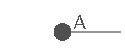
\includegraphics{graphics/concept/operations/CRE} &
  $ \emptyset $ & $ \rightarrow $ & $ A $ & &
  $ \emptyset $ & $ \rightarrow $ & $ A_N $ & &
  $ \emptyset $ & $ \rightarrow $ & $ A_T $ \\

  \midrule
  ICH & Identity Change & 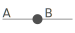
\includegraphics{graphics/concept/operations/ICH} &
  $ A   $ & $ \rightarrow $ & $ B $ & &
  $ A_N $ & $ \rightarrow $ & $ B_N $ & &
  $ A_T $ & $ \rightarrow $ & $ B_T $ \\

  \midrule
  CES & Cessation & 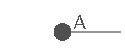
\includegraphics{graphics/concept/operations/CRE} &
  $ \emptyset $ & $ \rightarrow $ & $ A $ & &
  $ \emptyset $ & $ \rightarrow $ & $ A_N $ & &
  $ \emptyset $ & $ \rightarrow $ & $ A_T $ \\

  \midrule
  \multirow{3}{*}{UNI} &
  \multirow{3}{*}{Unification} &
  \multirow{3}{*}{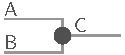
\includegraphics{graphics/concept/operations/UNI}} &
  $ A $ & $ \rightarrow $ & $ C $ & &
  $ A_N $ & $ \rightarrow $ & $ \emptyset $ & &
  $ A_T $ & $ \rightarrow $ & $ \emptyset $ \\
  & & &
  $ B $ & $ \rightarrow $ & $ C $ & &
  $ B_N $ & $ \rightarrow $ & $ \emptyset $ & &
  $ B_T $ & $ \rightarrow $ & $ \emptyset $ \\
  & & &
  & & & &
  $ \emptyset $ & $ \rightarrow $ & $ C_N $ & &
  $ \emptyset $ & $ \rightarrow $ & $ C_T $ \footnotemark \\

  \midrule
  \multirow{2}{*}{INC} &
  \multirow{2}{*}{Incorporation} &
  \multirow{2}{*}{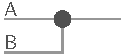
\includegraphics{graphics/concept/operations/INC}} &
  & & & &
  $ (A_N $ & $ \rightarrow $ & $ A_{N'}) $ & &
  $ A_T $ & $ \rightarrow $ & $ A_{T'} $ \footnotemark \\
  & & &
  $ B $ & $ \rightarrow $ & $ A $ & &
  $ B_N $ & $ \rightarrow $ & $ \emptyset $ & &
  $ B_T $ & $ \rightarrow $ & $ \emptyset $ \\

  \midrule
  \multirow{3}{*}{SEP} &
  \multirow{3}{*}{Separation} &
  \multirow{3}{*}{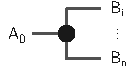
\includegraphics{graphics/concept/operations/SEP}} &
  $ A $ & $ \rightarrow $ & $ B $ & &
  $ A_N $ & $ \rightarrow $ & $ \emptyset $ & &
  $ A_T $ & $ \rightarrow $ & $ \emptyset $ \\
  & & &
  $ A $ & $ \rightarrow $ & $ C $ & &
  $ \emptyset $ & $ \rightarrow $ & $ B_N $ & &
  $ \emptyset $ & $ \rightarrow $ & $ B_T $ \\
  & & &
  & & & &
  $ \emptyset $ & $ \rightarrow $ & $ C_N $ & &
  $ \emptyset $ & $ \rightarrow $ & $ C_T $ \footnotemark \\

  \midrule
  \multirow{2}{*}{SEC} &
  \multirow{2}{*}{Secession} &
  \multirow{2}{*}{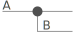
\includegraphics{graphics/concept/operations/SEC}} &
  $ A $ & $ \rightarrow $ & $ B $ & &
  $ (A_N $ & $ \rightarrow $ & $ A_{N'}) $ & &
  $ A_T $ & $ \rightarrow $ & $ A_{T'} $ \\
  & & &
  & & & &
  $ \emptyset $ & $ \rightarrow $ & $ B_N $ & &
  $ \emptyset $ & $ \rightarrow $ & $ B_T $ \footnotemark \\

  \midrule
  \multirow{1}{*}{NCH} &
  \multirow{1}{*}{Name Change} &
  \multirow{1}{*}{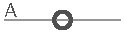
\includegraphics{graphics/concept/operations/NCH_TCH}} &
  & & & &
  $ A_N $ & $ \rightarrow $ & $ A_{N'} $ & &
  & & \\

  \midrule
  \multirow{2}{*}{BCH} &
  \multirow{2}{*}{Border Change} &
  \multirow{2}{*}{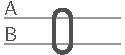
\includegraphics{graphics/concept/operations/BCH}} &
  & & & &
  & & & &
  $ A_T $ & $ \rightarrow $ & $ A_{T'} $ \\
  & & &
  & & & &
  & & & &
  $ B_T $ & $ \rightarrow $ & $ B_{T'} $ \footnotemark \\

  \midrule
  \multirow{1}{*}{TCH} &
  \multirow{1}{*}{Territory Change} &
  \multirow{1}{*}{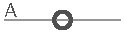
\includegraphics{graphics/concept/operations/NCH_TCH}} &
  & & & &
  & & & &
  $ A_T $ & $ \rightarrow $ & $ A_{T'} $ \\

  \bottomrule
\end{tabular}
\caption{Overview about all 10 historical geographic operations}
\label{tab:historical_geographic_operations}
\end{center}
\end{table}[H]

\addtocounter{footnote}{-4}
\footnotetext{$C_{T} = A_T \cup B_T$}
\addtocounter{footnote}{1}
\footnotetext{$A_{T'} = A_T \cup B_T$}
\addtocounter{footnote}{1}
\footnotetext{$B_T \cup C_{T} = A_T$}
\addtocounter{footnote}{1}
\footnotetext{$A_{T'} \cup B_{T} = A_T$}
\addtocounter{footnote}{1}
\footnotetext{$A_{T} \cup B_{T} = A_{T'} \cup B_{T'}$}

% paragraph historical_geographic_operations (end)

% - - - - - - - - - - - - - - - - - - - - - - - - - - - - - - - - - - - - - - -

combination of cases

There are topological rules rules that can be applied, e.g. two neighboring countries (polygons) share one common border (polyline). That preserves the relationship between them if their common border changes.

MECE principle: Mutually Exclusive and Collectively Exhaustive


A data model is an incomplete abstraction of the real world to develop a reasonable solution for the problem space.
Since the data model uses the concept of several existing one, it will derive also its name from it: The Hivent-Based Three-Domain Spatio-Temporal History Graph Data Model for Time-Stamped Vector Geometry
... or in short: HBTDSTHGDMTSVG

estd for vector graphics

3 domain model
identity: formal name of an entity

history graph model without changing state: active, inactive

simplification: just active / inactive, normal / contested + level of certainty

no transaction time, only valid / event time
only world time is regarded, not database time.


interior borders of countries, which are straight lines between manually defined border points.
=> vector model

A main problem is to maintain the integrity of the spatial topology when a new change gets inserted not at the end of the list. A simple example shows that problem: Given geo-object $X$ is part of the inital base configuration at change $t_b$. At a later change, e.g. $t_y$ $X$ gets replaced by object $Y$. If a new change that updates $X$ to $X'$ gets inserted before at time point $t_x < t_y$, then $t_y$ is not integer anymore, because object $X$ does not exist. That is why on insertion of a change, all succeeding changes have to be tested for integrity and it might be necessary to update later changes.

% \begin{figure}[ht]
%   \centering
%   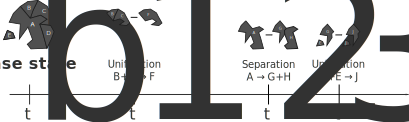
\includegraphics[width=0.8\textwidth]{graphics/basics/stdm/event-based_spatio-temporal_data_model}
%   \caption{The Event-Based Spatio-Temporal Data Model}
%   \label{fig:event-based_spatio-temporal_data_model}


\paragraph{possible extension} % (fold)
\label{par:possible_extension}

% paragraph possible_extension (end)

-> the whole earth is 100\% covered by spatial objects (full topology)
  countries, debated territories, unknown land, water
  Newtons concept of absolute space?


inclusion of universe $\Omega$:
CRE = SEC from $\Omega$
DES = INC into $\Omega$

% subsection historical_changes (end)


% section hivent_model (end)


store Hivents in DoublyLinkedList


% \subsection{Four-Domain Model}
\label{sub:four_domain_model}

According to the extension of the Three Domain model (see section \ref{sub:three_domain_model}), a spatio-temporal object can be represented separetely in the spatial, temporal and thematic domain. Additionally, the semantic domain uniquely identifies an object and is invariant. This applies to the concept of an Area that represents a country.


id: formal name

semantic: id (formal name)
spatial:  spatial attributes (territory)
temporal: Hivent -> HistoricalChange -> AreaChange
thematic: aspatial attributes (short name)

% subsection four_domain_model (end)

% ==============================================================================
\section{HistoGlobe} % (fold)
\label{sec:histoglobe}

Application: HistoGlobe
A distributed \emph{Web Information System}, consists of a remote server side, on which the storage and management of the actual data happens, and the client side on which the user communicates with the system. It hosts the user interface that is rendered in a Web browser.

map for spatial domain (x, y)
timeline for temporal domain (t)
-> 3D system

describe the components of the HG explicitally

ancestors successors
layers of administrative units
open to extension for additional attribute data (e.g. statistics)

requirements
  geographical knowledge
  contextualize / intersect historical sources
  accept imprecision
  prevent illusion of certainty

usable User Interface for both navigation and editing
-> problem: all interfaces are trés horrible!



% ------------------------------------------------------------------------------
\subsection{System Architecture} % (fold)
\label{sub:system_architecture}

The system developed in this thesis is Web-based. That means, there is a \emph{client}, a Web browser, and a remote Web \emph{server} with a database and a middleware. The Web browser hosts the applications user interface. If the user interacts with a tool the client sends a request to the Web server for new data. The middleware checks the request and queries the necessary data from the database. The data will be transformed and sendt back to the client. On the map and the timeline the new information will be shown.

This clear separation between the data (\emph{model}), the user interface (\emph{view}) and the middleware (\emph{controller}) follows directly from the \emph{model-view-controller pattern}: One part can be changed without interfering the other parts, e.g. if the 2D map is replaced by a 3D globe, only the view changes, but the middleware and the database can stay untouched. Likewise, the implementation of a new database technology has no consequences to the view.

% subsection system_architecture (end)


% ------------------------------------------------------------------------------
\subsection{Data Input} % (fold)
\label{sub:input}

This HGIS needs data about historical countries, their names and borders and historical events that lead to historical changes of these countries. There are a lot of free and open sources for geographic data about the current countries, their names and borders. One of the most exhaustive collections of geographic data in public domain is hosted by Natural Earth
\footnote{
  \textit{Natural Earth},
  URL: \url{http://www.naturalearthdata.com/downloads/},
  last access: 30.10.2015
}.
There is physical data (e.g. coastlines, rivers, or glacier areas) and cultural data (e.g. political borders, cities, roads, airports or timezones). OpenStreetMap also opens its database to the public
\footnote{
  \textit{Planet OSM},
  URL: \url{http://planet.openstreetmap.org/},
  last access: 30.10.2015
}.

However, data about historical countries and events are not as straightforward to aquire, because of the mostly qualitative nature of historical research (see section \ref{sub:history}). The most exhaustive free and open source of historical is the \emph{Wikipedia} and their article categories, e.g. \texttt{armistices} or \texttt{treaties}
\footnote{
  \textit{Category:Treaties},
  Wikipedia, the free encyclopedia,\\
  URL: \url{https://en.wikipedia.org/wiki/Category:Treaties},
  last access: 13.05.2016
}.
All sorts of historical events can be found, even translated into different languages. Some information is structured in information boxes, e.g. some historical treaties have a name, an image, a location, a signature and an effect date, an overview about treaty conditions and signatories. Particularily interesting for this thesis are articles about historical countries
\footnote{
  \textit{List of former sovereign states},
  Wikipedia, the free encyclopedia,
  URL: \url{https://en.wikipedia.org/wiki/List_of_former_sovereign_states},
  last access: 13.05.2016
},
because they contain the name of the country and meta information, e.g. their historical successors and predecessors. Building an open-source Historical Geographic Information System on the basis of Wikipedia would be a huge project with significant impact on the world of free and open education --- however, it would also be a big challenge: Wikipedia is incomplete, not all historical countries and events necessary to model the history of the world are available. It is also inconsistent, because not all articles about historical countries and events are structured, especially not to those who actually have an influence on a territorial change of a country, e.g. a border agreement. Retrieving, parsing and processing this information is a big challenge. Also the problem of accuracy and quality of information in the Wikipedia due to their open source nature has to be considered. Overall, using the Wikipedia as a data source for this thesis is not feasible, but is subject to further research.

% - - - - - - - - - - - - - - - - - - - - - - - - - - - - - - - - - - - - - - -
\paragraph{Historical maps} % (fold)
\label{par:historical_map}

The most problematic data to acquire is about the territories and borders of historical countries. There is no primary data source for that, so the only way to retrieve a border is to extract it from an historical map.

They also can be found on Wikipedia, or in historical map colletions, e.g. \emph{OldMapsOnline}. The project is developed ``out of a love of history and heritage of old maps'' and currently stores about 400000 historical maps
\footnote{
  \textit{Old Maps Online},
  URL: \url{http://www.oldmapsonline.org/},
  last access: 13.05.2016
}.
There are five steps to retrieve a border with points in geographic coordinates from an historical map.
\begin{enumerate}
  \item \textbf{Digitization}: If the map is on paper, it has to be scanned in the best possible quality. The result is a raster graphic.
  \item \textbf{Georeferencing}: The historical map has to fit as good possible on the reference map. This requires to manually define a set of reference points which are used to transform the map into the geographic coordinate system. This process is error-prone, especially if the projection of the historical map is not known and the map itself is not accurate
  \cite[pp. xvii]{knowles2002past}.
  The outcome is a raster graphic in which each pixel is assigned a geographic coordinate.
  \item \textbf{Preprocessing}: The raster image has to be be processed so that the desired border stands out and can be traced in the next step. This happens via greyscale conversion, thresholding or the Canny Edge Detector. This results in a monochrome graphic in which the desired border must be uninterrupted and clearly be seen.
  \item \textbf{Line detection}: By selecting a start and an end point of the border, the line gets traced automatically. This step vectorizes one particular feature, a borderline, from the raster graphic and produces a polyline in geographic coordinates.
  \item \textbf{Postprocessing}: In the last step, the polyline can be adapted: The line can be simplified to reduce unnatural artifacts and the position of border points can be manually edited. The final output of the whole process is a polyline whose points are expressed in the geographic coordinate system which can be used in the system as a border of an historic country.
\end{enumerate}

This process was developed in a preceding \emph{HiBo} project
\footnotetext{
  \textit{HiBo - semi-automatic extraction of borders from historical maps},
  Project of: B. Weber, N. K. Dankwa, K. Singh and T. Kashyappan, supervised by: Prof. Volker Rodehorst and Marcus Kossatz, Bauhaus-Universität Weimar, February 2015,
  URL: \url{https://bitbucket.org/bastian_weber/hibo},
  last access: 29.10.2015
}
(see figure \ref{fig:hibo}).

\begin{figure}[ht]
  \centering
  \begin{subfigure}{0.48\textwidth}
    \centering
    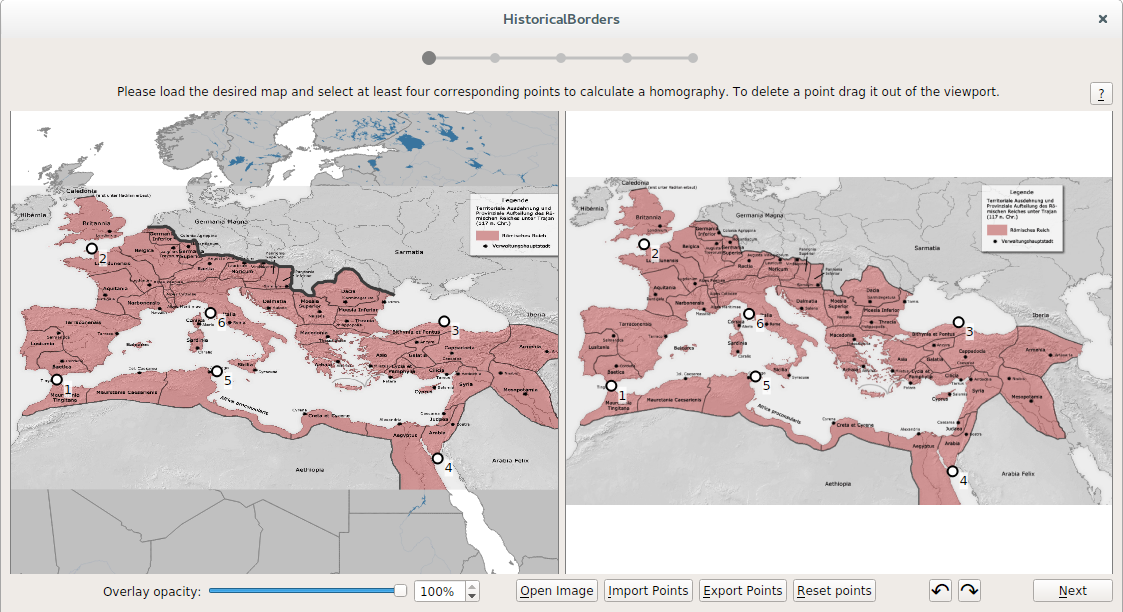
\includegraphics[width=0.95\linewidth]{graphics/basics/hibo1.png}
    \caption{Georeferencing}
  \end{subfigure}
  \begin{subfigure}{0.48\textwidth}
    \centering
    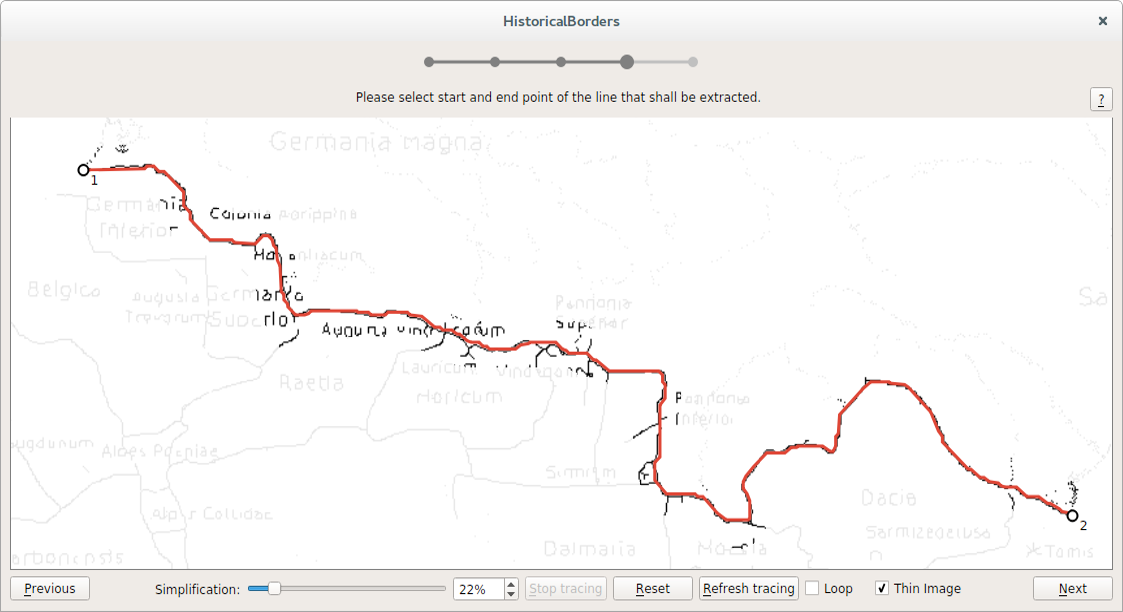
\includegraphics[width=0.95\linewidth]{graphics/basics/hibo2.png}
    \caption{Semi-automatic digitizing}
  \end{subfigure}
  \caption{Semi-automatic extraction of a border from a map of the Roman Empire \protect\footnotemark}
  \label{fig:hibo}
\end{figure}

% paragraph historical_map (end)


% - - - - - - - - - - - - - - - - - - - - - - - - - - - - - - - - - - - - - - -
\paragraph{Manual data input} % (fold)
\label{par:manual_data_input}

For the domain of this HGIS, the development of countries over time, there is no complete dataset available. Therefore, the system developed in this thesis needs to have an interface to enter historical data. The user needs to have an interface to enter information about historical events that change territories and names of historical countries. This data has to be acuired either from primary historical sources directly, or from free online sources. Next to Wikipedia, there are other collections of historical events, e.g. \emph{Correlates of War}
\footnote{
  \textit{Data Sets},
  Correlates of War,
  URL: \url{http://www.correlatesofwar.org/data-sets/folder_listing},
  last access: 13.05.2016
}
for quantitative data about international relations.
% paragraph manual_data_input (end)

% subsection data_input (end)



% ------------------------------------------------------------------------------
\subsection{Edit Mode} % (fold)
\label{sub:edit_mode}


user operations     CRE     UNI          SEP         TCH         NCH      DES
                     |      / \         /   \        /  \       /   \      |
HG operations       CRE   UNI   INC   SEP   SEC   TCH   BCH   NCH   ICH   DES

area changes        ADD   DEL*  DEL*  DEL   TCH   TCH   TCH   NCH   ADD   DEL
ADD, TCH, NCH, DES        ADD   TCH   ADD*  NCH?        TCH         DEL
                                NCH?        ADD*


geometries must be edited



% subsection edit_mode (end)

% ------------------------------------------------------------------------------
\subsection{HistoGraph} % (fold)
\label{sub:histograph}

% subsection histograph (end)

% section histoglobe (end)



% chapter concept (end)
%!TEX root = ../masters_thesis.tex

% ==============================================================================
  -> Managing Vagueness, Uncertainty and Granularity in Spatial Information Systems (VUG)
  %http://www.geos.ed.ac.uk/~gisteac/gis_book_abridged/files/ch13.pdf
  %http://link.springer.com/chapter/10.1007%2F978-3-642-14755-5_1
  %http://support.esri.com/en/knowledgebase/GISDictionary/term/uncertainty
  %http://www.geog.ucsb.edu/~kclarke/G176B/Lecture07.ppt
  -> Karl Grasser (Diss. Santa Barbara)
  -> Fuzzy, Imprecice,
  proabilities vs. possibilities

big problem: why? intention and motivation of author? hard to find out...
voice and perspective
medieval maps: natural landmarks as border points => inaccurate and imprecise
perspective: who is making the map? (illiterates?)
different names:
  US Civil War (North) vs.
  WWI (West) vs. Germanic War (Russia)
  WWII (West) vs. Great Fatherland War (Russia)

accepted uncertainty: date != exact timepoint, only D.M.Y
                      location != exact location, only name of place

\cite[chapter 2, p. 51]{solana2014spatio}

think about how to represent historical knowledge in geographic context
degree of certainty -> ironically: that has to be exact as well in a database table
=> reason: careful conclusions from historical maps

country borders
  coastlines
  interior
  disputed territories
    situation: n fully recognized countries and m non or partially recognized entities claim sovereignty over 1 territory
    territory is surrounded by disputed border
    question: does this disputed area claim sovereignty?
    \footnote \url{http://www.economist.com/blogs/economist-explains/2014/09/economist-explains-1}
  uncertain borders
    situation: n fully recognized countries commonly agree on a boundary between them, but the border is not clearly defined / fuzzy / uncertain
  states of borders
    planned
    agreed
    demarcated
    provisional
    valid
    vs. disputed

    borders: complex model: different states of boundaries: draft -> proposal -> dispute ->
    % \cite Wachowitz 1998 pp. 55


However, the first question arises regarding the relevance of the location: While the exact position of the battlefield of Verdun or the place where John F. Kennedy was assassinated might very relevant to the event itself, the location of a governmental bill, a declaration of independence or a border convention might not play an important role and usually happens in a representative place, e.g. the parliament or the office of a president. In a lot of cases, it is much more important which territories an event actually influences instead of where it happened.

Another constraint of the model is that it does only support coequal Areas and no hierarchies, e.g. a country consists of a set of states which consist of a set of counties. Also, independent Areas that overlap other areas, e.g. to visualize a disputed zone or the expansion of the rain forest, are not possible given the model.

\paragraph{Hierarchical Areas} % (fold)
\label{par:hierarchical_areas}

CTR -> STA -> CTY -> CIT
each level one layer
aggregate geometry upwards

% paragraph hierarchical_areas (end)

\paragraph{Overlapping Areas} % (fold)
\label{par:overlapping_areas}

e.g. war zone,
independent layer

% paragraph overlapping_areas (end)


% ==============================================================================


\chapter{Uncertainty} % (fold)
\label{cha:uncertainty}

Every aspect of the concept (chapter \ref{cha:concept}) and the development (chapter \ref{cha:development}) of this work is based on the prerequisite of full certainty of the data. That means both the Historical-Geographic Operations and the Hivent-Based Spatio-Temporal Data Model assume that the dates of the historical events, the names and territories of the historical and current areas and the historical relations between events and areas are accurate and reasonably precise (definitions see \ref{sec:types_of_uncertainty}).

However, this assumption is far from valid. In historical research, uncertainty is one of the major problems (see \ref{sub:history}) a historian has to deal with on a daily basis: sources, even primary sources, can be biased towards the author of the source, information can be imprecise or even inaccurate and information can be conflicting with other sources. This chapter explains problems with uncertainty in the domain of development of countries in time and space and develops approaches to deal with these problems.


% ==============================================================================
\section{Definition of a Country} % (fold)
\label{sec:definition_of_a_country}

The problem begins with the definition of a term that almost everybody in the world is familiar with: a ``country''. Since countries are the domain of this historical geographic information system, it must be possible to decide for each current and historic territorial entity in the world if it is or was a country or not. Therefore a clear and non-conflicting definition of a country is necessary. However, this is impossible to do.

The Oxford Dictionary definition of a country reads as follows:
\begin{quote}
  ``The \emph{territory} of a \emph{nation}; a \emph{region} constituting an \emph{independent state}, or a region, province, etc., which was once independent and is still distinct in institutions, language, etc.''
  \footnote{\textit{country, n. and adj}, Oxford English Dictionary, URL: \url{http://www.oed.com/view/Entry/43085?}, last access: 2016-04-25}
\end{quote}

This definition includes many different concepts and terms: the territory or region that the country is on, a nation or state, a population and a culture of the territory in terms of institutions or languages. While nation and state are commonly used as synonyms for countries, their meaning varies from case to case, as it will be examined in this section.

To understand what a country really is, the United Nations as an intergovernmental organisation are a valuable source. It was found after World War II (October 1945) and promotes international peace keeping, security, protection of human rights or humanitarian aid to all its member states which should coincide with all the countries in the world. The committee currently has 193 full member states and two permanent obervers: The Holy See (Vatican City) and the State of Palestine \cite{UNmembers}. But these 195 members in total do not cover all places in the world -- and also a membership in the United Nations does not mean that the question of statehood can simply be answered.

% ------------------------------------------------------------------------------
\subsection{Special Cases} % (fold)
\label{sub:special_cases}

Examining the list of the UN member states yields several interesting observations and special cases, which can be classified by their membership status in the United Nations and their degree of international recognition.


\paragraph{UN observer states} % (fold)
\label{par:un_observer_states}

The \emph{Holy See} is the juridcal and spiritual entity representing the territory of Vatican City. It is a fully recognized and sovereign state but is not a full member of the UN, because it has never applied for it. It is the by far smallest sovereign state in the world (0.44 m²), is an enclave inside the city of Rome with a population of only 800 people, including 30 women \cite{VaticanPopulation}.

The \emph{State of Palestine} has a population of 4.8 million people \cite[as of 2016]{PalestinePopulation} and is also an UN observer state. However, it is totally different in terms of sovereignty: While it consists of the territories of the West Bank, East Jerusalem and the Gaza Strip, their borders were drawn in the 1949 Green Line Armistice Agreement but were never intended to be used as international boundaries \cite{PalestineTerritory}. Since then, the ongoing and complex conflict with the State of Israel lead to a difficult situations regarding the sovereignty over the territories. Therefore, the state has no clearly defined territoy. Moreover, while 114 states officially recognize the Palestinian state, almost all current main economic powers do not, including the Canada, France, Germany, Italy, the United Kingdom and the United States. None of them even voted in favor of Palestine receiving an observing status in the UN \cite{PalestineUN}. That means, unlike the Holy See, Palestine is not a fully sovereign and recognized state.

% paragraph un_observer_states (end)

\paragraph{UN non-members with limited recognition} % (fold)
\label{par:un_non_members_with_limited_recognition}

\emph{Kosovo} is a state Europe and and declared independence from Serbia in 2008. It has a clearly defined territory and a permanent population and is recognized by 111 UN member states. In order for Kosovo to become a full member of the United Nations, all permanent members of the security council (United Kingdom, France, Russia, China and the United States) must agree. But since Russia and China strongly support the territorial integrity of Serbia, they would veto Kosovos membership in the United Nations. Therefore, Kosovo is not even an observer state of the United Nations, although having about the same degree of international recognition as Palestine \cite{KosovoThanksYou}.

The status of Taiwan is a very complicated issue. An overgeneralized description of the problem, which involves two territories and two political entities, is: There is the \emph{People's Republic as China} (commonly known as China), with full control over mainland China, and the \emph{Republic of China}, governing the island of Taiwan. However, both political entities claim each others land. That means, there are two states claiming the exact same territory. But, since 1971 the People's Republic of China is the representative of whole China in the United Nations, including the island of Taiwan. Because it is part of the Security Council, it successfully vetos membership requests of the Republic of China. Therefore, it can not be a member of the United Nations, although it operates like an independend country by international standards: They have an own jurisdiction, issue own passports and have unofficial diplomatic relations to most countries in the world. But officially, only 22 member states of the United Nations uphold diplomatic relations to Taiwan \cite{TaiwanRecognition}. To all of these states the People's Republic of China does not have any diplomatic relations, which makes also them an only partially recognized state.

There are other non-member states of the United Nations which have not yet gained broad international recognition: the Sahrawi Arab Democratic Republic (recognized by 84 UN member states \cite{WesternSaharaRecognition}), Abkhazia (6 \cite{AbkhaziaRecognition}), South Ossetia (5 \cite{SouthOssetiaRecognition}), the Turkish Republic of Northern Cyprus (1 \cite{NorthernCyprusRecognition}), Nagorno-Karabakh Republic (0 \cite{NagornoRecognition}), Transnistria (0 \cite{TransnistriaRecognition}) and Somaliland (0 \cite{SomalilandRecognition}).

% paragraph un_non_members_with_limited_recognition (end)

\paragraph{UN members with limited recognition} % (fold)
\label{par:un_members_with_limited_recognition}

In addition to the Republic of China, there are five other member states of the United Nations that are not fully recognized by all other UN members: Armenia (not recognized by Pakistan \cite{ArmeniaRecognition}), the Republic of Cyprus (not recognized by Turkey \cite{CyprusRecognition}), North and South Korea (officially Democratic People's Republic of Korea and Republic of Korea, mutual non-recognition \cite{KoreaRecognition}) and the State of Israel, which 32 UN member states do not recognize \cite{IsraelRecognition}.

% paragraph un_members_with_limited_recognition (end)

\paragraph{Special Territories} % (fold)
\label{par:special_territories}

Additionally to countries gaining for international recognition there are territories belonging to fully sovereign countries with a varying degree of sovereignty. For example Greenland is an autonomous country within the Kingdom of Denmark, but not a  sovereign state and therefore not a member of the United Nations. The same applies to the Faroer Islands (part of Denmark) and numerous overseas territories of the United Kingdom, the French Republic and the Kingdom of the Netherlands in the Carribean, the Indian Ocean or the Southern Pacific Ocean. Moreover, there are five quasi-independent countries in a so called \emph{Free Association}: Niue and Cook Islands are associated to New Zealand and not part of the United Nations. The Marshall Islands, the Federated States of Micronesia and Palau are associated to United States, but in contrast are full UN members \cite{SpecialTerritories}.

% TODO?
% example United Kingdom:  country?
% difference clear: geography             politics
%                   British Isles         United Kingdom of Great Britain and NI
%                     Great Britain         Scotland, England, Wales, Northern Ireland (province)
%                     Ireland             Republic of Ireland
%                     Shetland Islands
%                     Isle of Men
%                     ...

% Scotland, England and Wales are countries, but not sovereign states, Northern Ireland is a province and not a country. The UK is a constituent country, just like the Kingdom of the Netherlands and the Kingdom of Denmark.

% paragraph special_territories (end)

This incomplete and simplified list of special cases manifests the big problem that is associated with the terms ``country'', ``state'' or ``nations'': There is neither a \emph{de jure} consistent definition nor a \emph{de facto} consistent usage of these terms. Everything breaks down to two different concepts:


% subsection special_cases (end)

% ------------------------------------------------------------------------------
\subsection{Declaratory vs. Constituitive Theory} % (fold)
\label{sub:declaratory_vs_constituitive_theory}

The declaratory theory, established in the Montevideo Convention 1933 \cite{MontevideoConvention}, gives each entity the right to declare a state if it matches all of the four requirements:
\begin{compactenum}
  \item a clearly defined territory
  \item a permanent population
  \item a political representation / government
  \item the \emph{capacity} to enter diplomatic relations
\end{compactenum}

These four requirements make sure that a state can exist physically and politically. However, it is worth noticing that this definition does not include any actual diplomatic relations to other states, but only the capacity to enter them. Therefore the existance of a state is independent from its recognition by other states. In other words: ``A country is a country when it thinks it is a country.''

In contrast, the constituitive theory requires exactly that: A state can only be considered as such if it is recognized by other states. However, it is not defined anywhere by how many other states \cite{StateTheory}. In short: ``A country is a country when other countries think that country is a country.'' \cite{greyCountries}

\begin{figure}[ht]
  \centering
  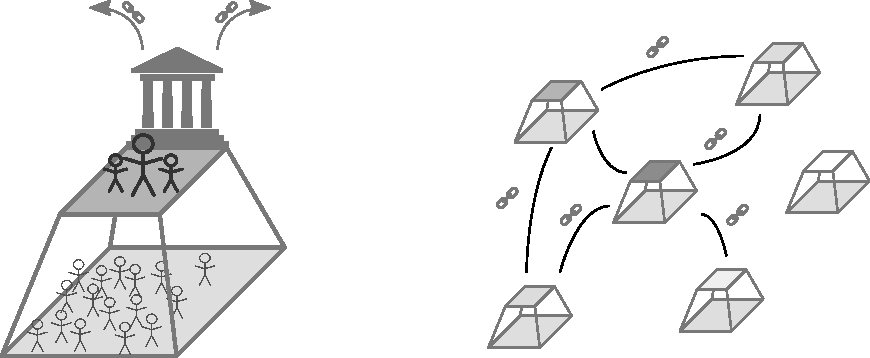
\includegraphics[width = 0.8\textwidth]{graphics/uncertainty/decl_const_theory}
  \caption{The Declaratory Theory (left) and the Constituitive Theory (right) of Statehood}
  \label{fig:declaratory_constituitive_theory}
\end{figure}

Both theories have advantages and disadvantages, but the two main problems are:
\begin{enumerate}
  \item Following the declarative theory, countries are self-classifying and potentially conflicting entities. The application of this measure would grant Kosovo, the Republic of China, Abkhazia or the Sarhawi Arab Democratic Republic full statehood. However, since their territories are contested, this would lead to overlapping territories with Serbia, China, Georgia and Morocco, which is impossible.
  \item There is no superior organization that can judge if a country is a country or not. Even the United Nations fail to do so, because their membership requirements prevent states like Kosovo or the Republic of China from becoming full members. They also have no power to rule out problems regarding the independence of Transnistria or Somaliland.
\end{enumerate}

Therefore it is impossible to objectivly classify an area as a country or not: nobody can say if Kosovo, the State of Palestine or Niue are countries or not. These theories have been introduced in the previous 80 years. For the time before that, a conflict-free decision of what is country is not just impossible, but also not justifyable because of a lack of jurisdiction.

That means, an historical geographic information system with the goal to visualize the development of the countries on Earth in time and space inevitably deals with uncertain information that certain parties see as wrong. Its data model can not perfectly fit self-classifying data and can not rely on an objective data source. The system has to contain approaches that deal with this problem.

% subsection declaratory_vs_constituitive_theory (end)

% section definition_of_a_country (end)


% ==============================================================================
\section{Types of Uncertainty} % (fold)
\label{sec:types_of_uncertainty}

In order to understand different types of uncertainty it is important to understand the concepts of \emph{disagreement}, \emph{precision} and \emph{accuracy}.

The model in an information system tries to resemble the real world as good as possible and necessary -- in this case the history of countries. If there is already a conflict in the real world, e.g. the Kasmir region which is claimed by both India and Pakistan as part of their territory, then this is a \emph{disagreement} which also has to be proberly modeled as such in the system.

The better a model simulates the reality, the more \emph{accurate} or correct it is. That means, the closer it gets to the target, the higher is the accuracy. \emph{Precision} or exactness describes how similar the results are compared to each other, independent from the distance to the target. That means a precise model gets the same results over and over again (see figure \ref{fig:accuracy_precision}).

\begin{figure}[ht]
  \centering
  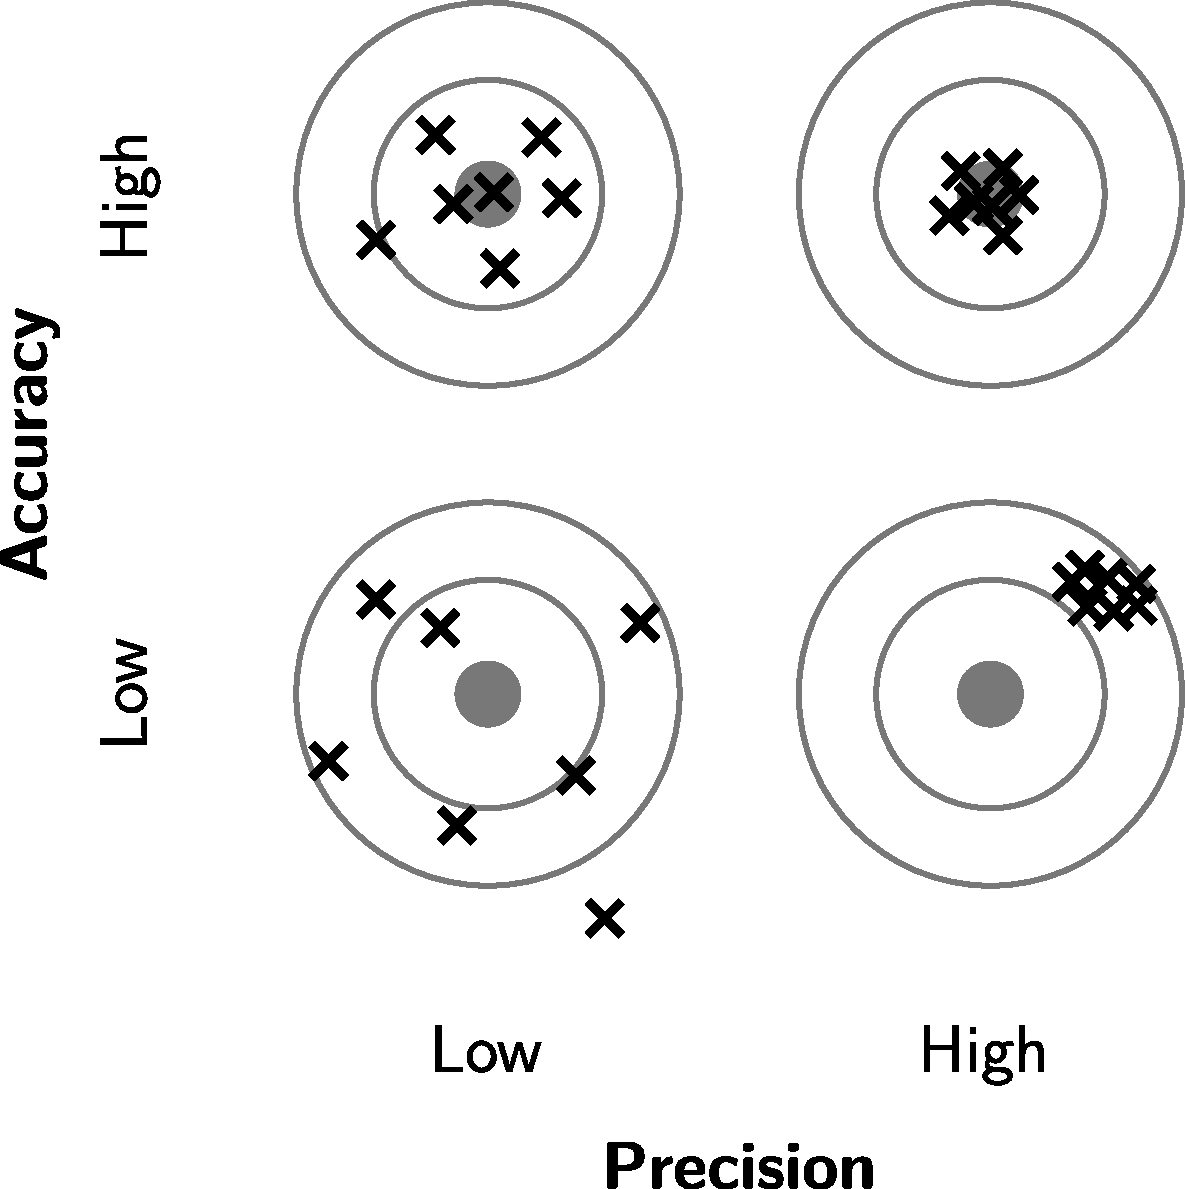
\includegraphics[width = 0.35\textwidth]{graphics/uncertainty/accuracy_precision}
  \caption{The difference between accuracy and precision}
  \label{fig:accuracy_precision}
\end{figure}

If the border between the Principalities of Transsylvania and Wallachia is deducted from an historical map of 1600, the course of the border is is inaccurate to a certain degree, because the map does not show the real world correctly. However, it can be modelled in the system very precisely, because the coordinates of the border points are stored as floating point numbers in the data model. In contrast, there is currently no agreement upon territory of Palestine, although the different versions can be modelled very precisely. In order for the model to also be accurate in this case, it would need to support contested territories.

Hereafter the current data model introduced in section \ref{cha:development}
% TODO: reference to actual section with the data model
is evaluated in terms of accuracy and precision.


\paragraph{Hivents} % (fold)
\label{par:evaluation_hivents}

The model for historically significant happenings contains only the following meta information: name, date and location of the event. This has several shortcomings in terms of precision:

The name of an historical event can have different versions: a long, official version and a short common version. The commonly known ``Treaty of Versailles'' (1919) is officially called the ``Treaty of Peace between the Allied and Associated Powers and Germany''. Also the name is different in other languages affected by the treaty. Additionally, there can be different versions of the name from different perspectives, even within the same language, e.g. the ``American Civil War'' as it is known today was alternatively called ``War Between the States'', ``War for Southern Independence'' or ``War of Northern Aggression'' depending on the perspective.
The ~\texttt{Hivent}~ model does not account for different languages and versions and is therefore not very precise.

The ~\texttt{Hivent.date}~ is supposed to represent the temporal dimension of an historical event. While an historical change itself is discrete and happens at exactly one time point, the historical event yielding this change might not. The ``Congress of Vienna'' which reordered the empires on the European mainland was one of the main historical events in modern European history. While the changes of the congress came into effect on 9. June 1815, the congress itself took place in Vienna from September 1814 until June 1815 which is also a timespan of interest. Another phenomenon becomes apparent in the ``Convention for the Extension of Hong Kong Territory'' (1898) which had a predefined length of 99 years. The treaty therefore has two dates in which historical changes happened: the date the treaty came into effect (Hong Kong becomes part of the United Kingdom) and the date it stopped being in effect (Hong Kong is handed over to China). Other interesting aspects are different calendar systems used in different parts of the world throughout history: the October Revolution in Russia (1917) happened in November in their Gregorian Calendar system, but in October in the Julian Calendar. Also timezones can play a crucial role: The German Instrument of Surrender ending World War II in Europe came into effect on 8. May 1945 at 23:01 Central European Time, so the 8. May is celebrated as the Victory Day in Western Europe. But in the Soviet Union and nowadays Russia that happened at 1:01 Moscow Time on 9. May 1945 which is why the celebration of the Victory Day there happens one day later. While the ~\texttt{Hivent.date}~ field in the data model works with timezones, it does not support different calendar systems or multiple dates associated with one ~\texttt{Hivent}~ which limits its precision.

The event location is represented by the ~\texttt{Hivent.location}~ name of a place, which can e.g. be a city, a battlefield or a region. The model is not very precise, because the actual geospatial location or region in which an historical event happened is not stored in the system. Additionally, it does not support names in different languages.

The even larger problem is an integral lack of accuracy: The whole nature of historical research is based on subjective interpretation of supposedly objective primary sources. But it is questionable if a source can actually be objective. Each bill, treaty or speech is written by somebody, each map was drawn by someone and has therefore a subjective note. Information in a primary source can be (un)intentionally incomplete, imprecise or inaccurate. The source can be biased towards the author, can contain secret passages not open to the public or its geographic information might be wrong. There are many problems involved in historical sources which makes the acquisition of objective historical data almost impossible. The further documents go back in time, the lower is the expected accuracy. Since all the information in the historical geographic information system is based on primary sources, the data in the system inherits these problems.

% paragraph evaluation_hivents (end)

\paragraph{Areas} % (fold)
\label{par:evaluation_areas}

Also the model of an abstract area, consisiting of a territory and a name, is problematic in terms of accuracy and precision. As it has been discussed in subsection \ref{sec:definition_of_a_country} in detail, it is impossible to objectively model all areas free of conflicts. But the current model does not support the status of a territory as being contested Also, countries can be part of other autonomous (constituent) countries, like England is part of the United Kingdom of Great Britain and Northern Ireland or Greenland is part of Denmark. However, the data model does not support different levels of sovereignty, autonomy or international recognition.
% Additionally the historical context acquired by the start and end change that created or destroyed the ~\texttt{Area}~ can be ambiguous. While the motvation was to historically connect different countries to form an historical graph, the automatic deduction of historical succession from the historical geographic operations might not accurately replicate the identity of a state. An example is the German Democratic Republic which both historically and geographically seems to be a decendent of Allied-occupied Germany after World War II and therefore an indirect successor of the German Empire. However, the constitution of the GDR emphazised
% TODO: source? -> Berno
% think about it: is it really the case?

The ~\texttt{AreaName}~ has the same problem than the ~\texttt{Hivent.name}: it differs among the languages or even among cultures using the same language. The model does not support that. But in one aspect it is more precise than for historical events, because it contains both the formal and the short name of a country.

More problematic is the ~\texttt{AreaTerritory}: Areas bordering international water have a constant coastline assuming that it has never changed. This is inaccurate, because coastlines gradually change all the time, therefore also the boundaries of the countries. The data model does support neither that nor international sea borders which are parts of a countries territory. The primary source for territories of countries are historical maps. They show the status of a country at one point in history or sometimes a territorial change. The process of extracting a boundary from an historical map is error-prone and yields to a loss of accuracy in each step on the way: digitizing, georeferencing and contour tracing. The level of inaccuracy depends on the resolution, the map projection and the colors used in the map. In the data model it is not possible to provide information about the expected accuracy of a territory.

Another problem is that the territory is stored as a whole polypolygon. Different parts of the border can have a different status, e.g. one part is a sea border, one is a well-established and demarcated border to neighboring country X and another part is a contested border to neighbour Y. The ~\texttt{AreaTerritory}~ data model does not account for these differences.

Accurately modelling contested territories is also problematic. It is based on the principle that there can not be overlapping territories at the same time. That means, a contested territory, for example China or occupied territories in the State of Palestine by the State of Israel can only exist once at the same time and therefore have to treated specially. But the data model does not support contested areas. To go even further, it is questionnable which areas should be included in the data model and which not. While it seems obvious to have Spain, Saudi-Arabia and Azerbaijan in the system, the question of whether or not to include the State of Palestine, Abkhazia, Somaliland or micronations like the Conch Republic in the Florida Keys is hard to answer.

% paragraph evaluation_areas (end)

Overall, the current data model poorly accounts for different levels of uncertainty in historical geographic information: imprecise and inaccurate sources, different viewpoints and interpretations, contested territories, changing coastlines or different languages. The question of the upcoming subsection is: How can the data model be extended in order to be more accurate and more precise?


% section types_of_uncertainty (end)

% ==============================================================================
\section{Solution Approaches} % (fold)
\label{sec:solution_approaches}

In summary, the shortcomings of the current concept are:

\begin{enumerate}
  \item General
  \begin{enumerate}
    \item only one language (English)
    \label{problem_general_multilang}
    \item constant coastlines
    \label{problem_general_coastlines}
  \end{enumerate}
  \item Hivent
  \begin{enumerate}
    \item only one historical perspective on the Hivent name
    \label{problem_hivent_perspective}
    \item only one discrete Hivent date
    \label{problem_hivent_dates}
    \item only one calendar system (Julian Calendar)
    \label{problem_hivent_calendar}
    \item only location name, no connection to the map
    \label{problem_hivent_location}
  \end{enumerate}
  \item Area
  \begin{enumerate}
    \item only one historical perspective on the Area name
    \label{problem_area_perspective}
    \item all Areas on the same level (no dependencies)
    \label{problem_area_levels}
    \item no support for non-sovereign autonomous regions
    \label{problem_area_autonomy}
    \item no credibility of Areas existence (via international recognition)
    \label{problem_area_recognition}
    \item only clear territories, no support for neutral zones or contested territories
    \label{problem_area_territory}
    \item no support for uncertain parts of a territory
    \label{problem_area_territory_certainty}
    \item no support for international sea borders
    \label{problem_area_territory_sea_borders}
  \end{enumerate}
\end{enumerate}

A higher accuracy in the data model usually leads to a higher complexity. This trade-off has to be thoroughly taken into consideration when supporting a new feature to make a model more accurate. This is why the following problems will be ignored in the rest of the thesis:
\begin{itemize}
  \item [\ref{problem_general_coastlines})] Coastlines change continuously, therefore the Hivent-Based Spatio-Temporal Data Model is not suitable. A support for coastline changes would require another data model applied to coastlines. This is out of the scope of this thesis. One approach is to model international waters just like any other area with a name and a territory and change the boundaries according to an underlying continuous function. This way, the countries sharing that coastline as their international border would change likewise.
  \item[\ref{problem_hivent_perspective})] The support for different historical perspectives on the same event, e.g. different names and descriptions or even different historical changes would create a research tool with great potential. It would enable the possibility for different versions of history based on alternative scenarios (``What if X would have (not) happened?''). However, this would significantly increase the complexity of the system and would also be very subjective.
  \item[\ref{problem_hivent_calendar})] The introduction of different calendar systems would not increase the accuracy of the model significantly. The dates in the system must all stick to the Julian calendar, which is a reasonable requirement to avoid unnecessary complexity.
  \item[\ref{problem_area_perspective})] see \ref{problem_hivent_perspective})
  \item[\ref{problem_area_territory_sea_borders})] Currently each countries territory extends in a range of 3 to 12 miles (5 to 20 kilometers) \cite{UNSeaBorders} into international waters. While this is important to accurately model a territory, it is complex, because not every country has signed the convention and each signing party can choose their range into international water. %TODO: is that true?
  This would not just increase the complexity of the model but also create unfamiliar country territories.
\end{itemize}

In order to tackle the remaining shortcomings of the current concept, both the user interface and the data model have to be extended.

% ------------------------------------------------------------------------------
\subsection{Extension of the Edit Mode} % (fold)
\label{sub:extension_of_the_edit_mode}

Two new operations (see figure \ref{fig:edit_mode_extension}) are introduced: \texttt{SCH} changes the status of an area and \texttt{REC} declares a new recognition, i.e. one country internationally recognizes another one.

\begin{figure}[ht]
  \centering
  
\includegraphics[width = 0.6\textwidth]{graphics/uncertainty/edit_mode_extension.png}
  \caption{Newly designed and extended buttons for edit operations.}
  \label{fig:edit_mode_extension}
\end{figure}


\paragraph{Set New Territory} % (fold)
\label{par:set_new_territory}

Also the edit operation workflow gets changed. The second step (\texttt{SET\_NEW\_TERR}) defines the territory of the new area(s). Instead of drawing the whole territory as a set of polygons, the user draws one borderline at a time, geometrically as a polyline. This has the main advantage that each part of the border is treated separately.

The borderline is assigned a degree of certainty, in the interface controlled by a horizontal slider, in the model as a certainty value (\texttt{certainty} $\in~]0 .. 1]$). Absolute certainty ($1.0$) creates a sharp and crisp line on the map. In case of uncertainty (\texttt{certainty} $\in~]0..1[$) three different visualization methods are introduced:

\begin{enumerate}
  \item Blurred Border: The higher the uncertainty, the wider and more blurry the border.
  \item Border Corridor: With increasing uncertainty, the offset around the actual border line extends. That creates a corridor in which the actual border is probably in.
  \item Blurred Border Corridor: The combination of the first two approaches.
\end{enumerate}

A simple model for the calculation of the blur factor, line width and offset distance is:
\begin{center}
\begin{math}
    f(c) = -1 \cdot S \cdot ln(c) + I
\end{math}
\end{center}
where $c$ is the certainty factor, $S>0$ is a scaling factor and $I$ is the inital value (for width: $1~px$, for blur: $0$, for offset: $0~px$). In the example in figure \ref{fig:uncertainty_border} the scaling factor $S=4$. In the Blurred Border Corridor method, the scaling factor for line width and the blur factor was halved. Further analysis and user testing are required in order to decide for one of the three approaches to be used in the system.

\begin{figure}[H]
  \centering
  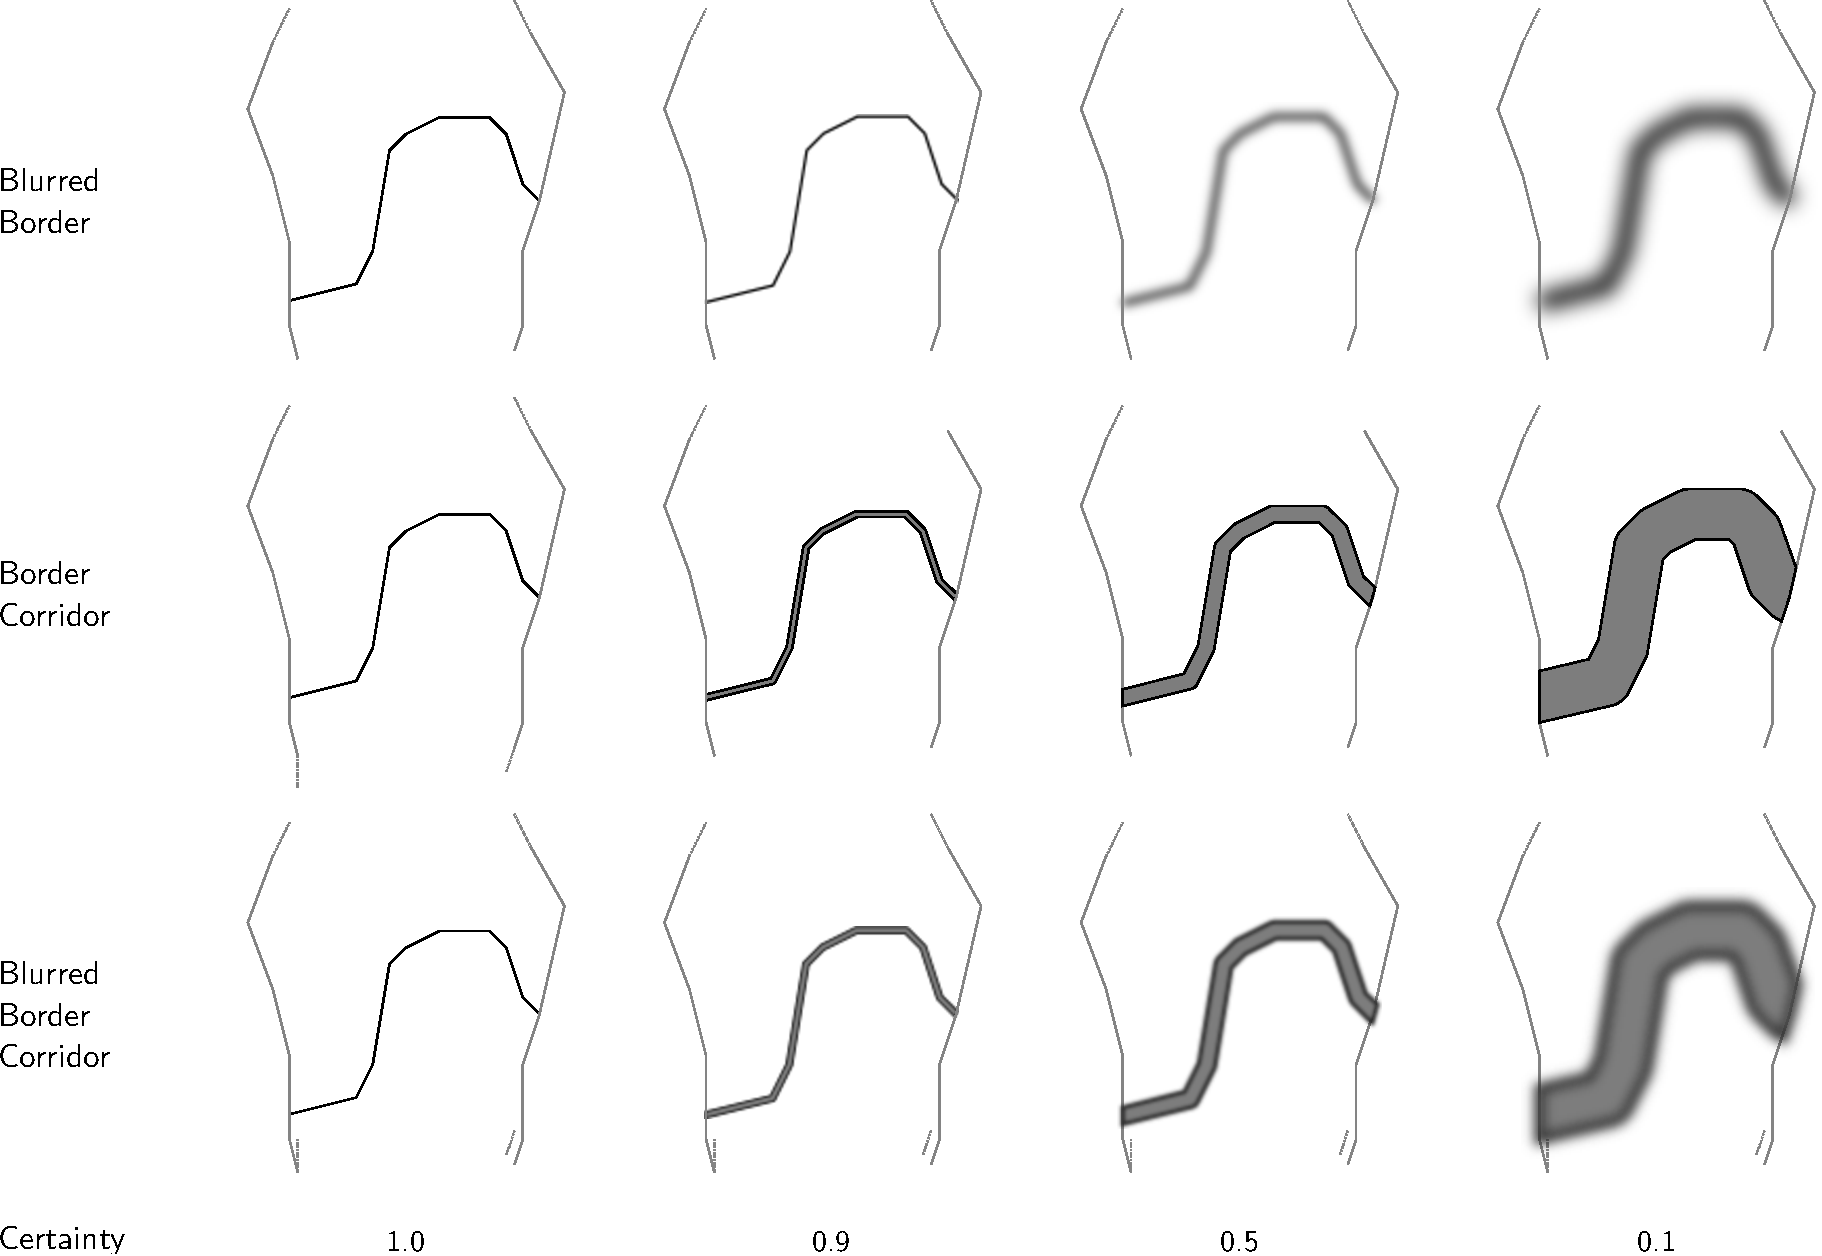
\includegraphics[width = 0.8\textwidth]{graphics/uncertainty/border}
  \caption{Three different methods to visualize uncertain courses of a border}
  \label{fig:uncertainty_border}
\end{figure}

Another advantage of the input of borderlines instead of territories is that once the model is further advanced, coastlines can be continuously changed according to an appropriate change model (see problem \ref{problem_general_coastlines}). This can be applied solely to the coastlines without affecting the interior borders.

A new border point automatically snaps to an existing border point, if the mouse position is close enough to it (an appropriate threshold might be $5~px$). This allows for a smooth workflow and is required to create closed polygons. In case the borderline is closed, it gets treated as a complete polygon and territory. When the user finished a territory by defining all surrounding polylines that create a closed ring, the polygon gets assembled. If a borderline meets another borderline at an interior node, the polyline gets split up into two parts so that each meeting point of borders is the start or end point of a polyline. This way integrity is maintained and each territory compounds of several polylines creating a set of closed polylines: a polypolygon.

\begin{figure}[H]
  \centering
  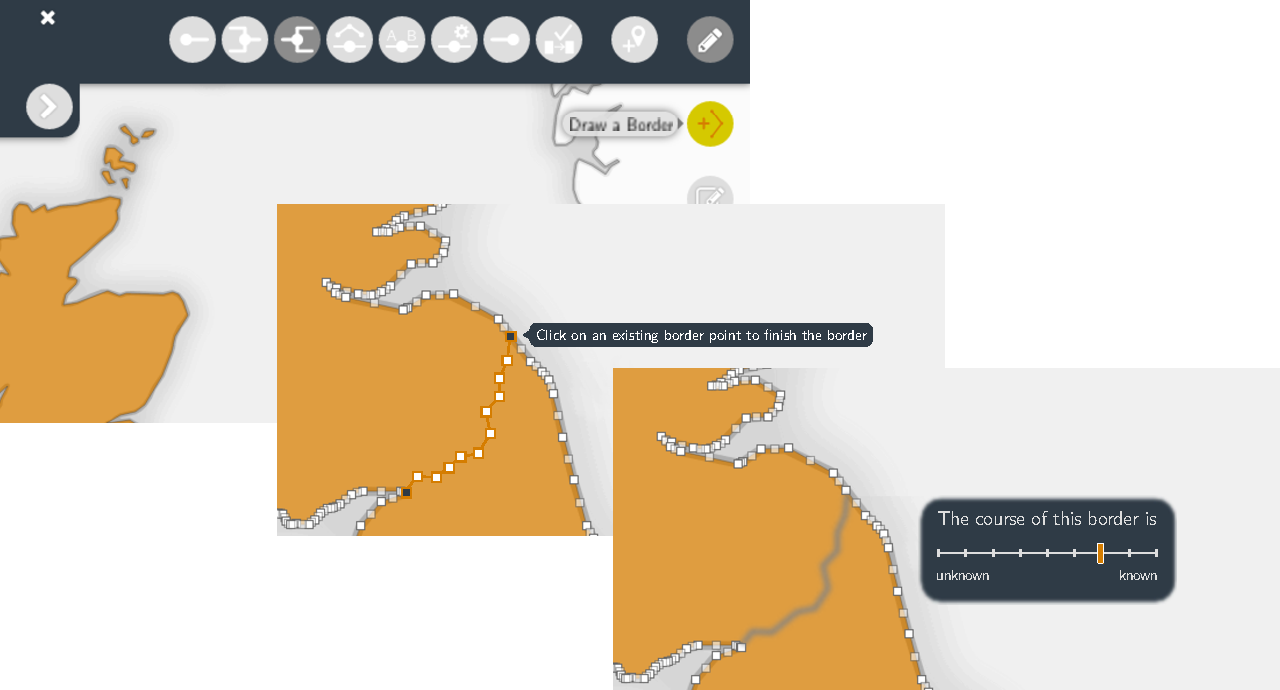
\includegraphics[width = 0.8\textwidth]{graphics/uncertainty/new_territory_tool}
  \caption{Drawing historical borders instead of full areas and definining a level of certainty.}
  \label{fig:uncertainty_new_territory_tool}
\end{figure}

If the created territory overlaps with an existing territory, its intersection will created a separate territory. In the next step, this territory can then be defined as a contested area or defined as a part of another area. If the step yields an empty territory that was claimed before, it can later be defined as a neutral zone or unclaimed land.

% paragraph set_new_territory (end)


\paragraph{Set New Name} % (fold)
\label{par:set_new_name}

When defining the name of an area, the user will get actual name suggestion. These result from a collection of current and historical countries from Wikipedia. That saves time for researching short and formal names of areas. In the long run, the system can be synchronized with Wikipedia or even be designed as an extension for Wikipedia articles about current or historical countries.

\begin{figure}[H]
  \centering
  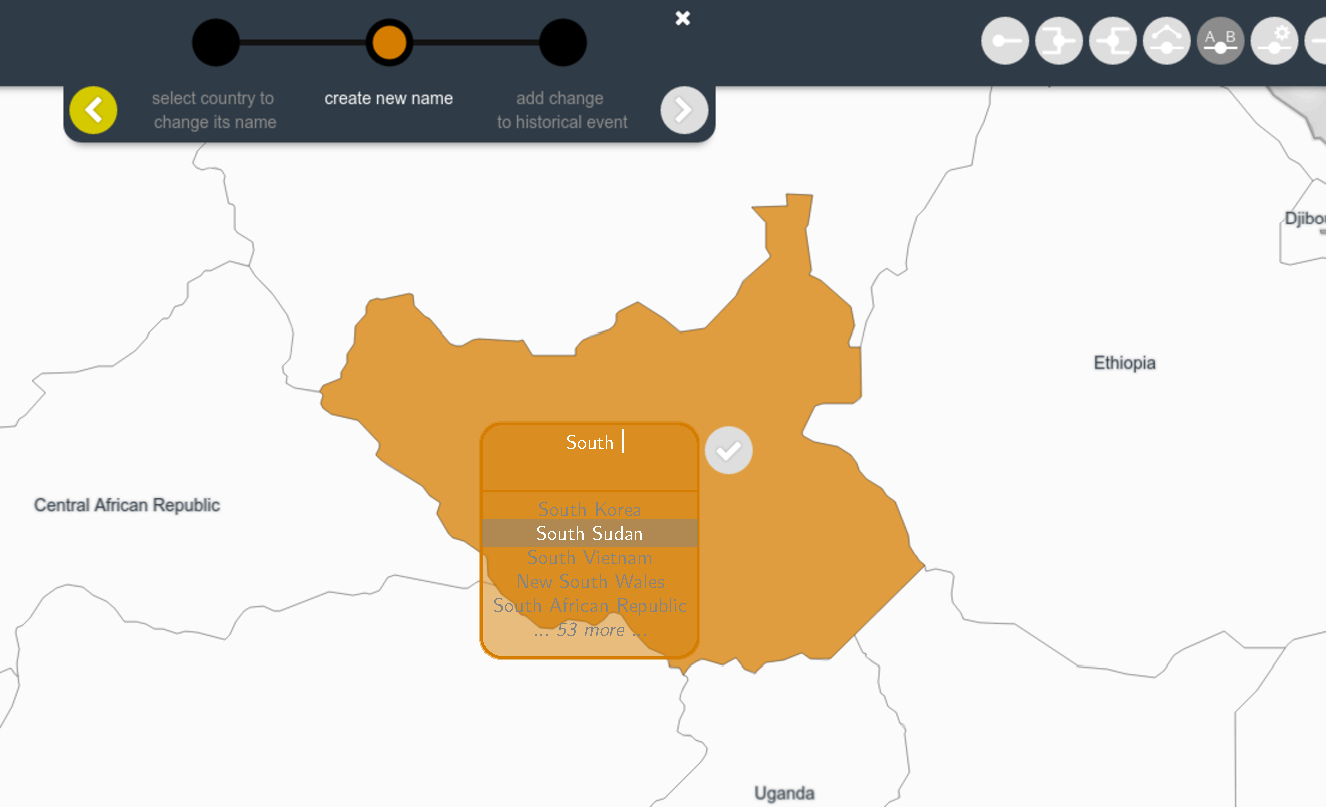
\includegraphics[width = 0.8\textwidth]{graphics/uncertainty/new_name_tool}
  \caption{Getting suggestions for the name name from Wikipedia.}
  \label{fig:uncertainty_new_name_tool}
\end{figure}

% paragraph set_new_name (end)

\paragraph{Set New Status} % (fold)
\label{par:set_new_status}

To treat special areas differently, a new step in the edit operation workflow gets defined. After the territory and the name of a new area are defined, a special status can be assigned to it:

\begin{enumerate}
  \item A \emph{fully sovereign country} is a political entity with full sovereignty over its territory and people and significant international recognition, e.g. Estonia.
  \item An \emph{unclaimed land} is a territory that is not claimed by any political entity, e.g. currently Antarctica.
  \item A \emph{neutral zone} is often a buffer zone between two conflicting countries, e.g. the UN Buffer Zone in Cyprus.
  \item A \emph{contested territory} is claimed by at least two different political entities of the same hierarchical level, e.g. the Kashmir region between India and Pakistan. It is also suitable for areas that have claimed independence from a sovereign country but are not yet regonized as such, making their whole territory contested, e.g. Nagorno-Karabakh (see figure \ref{fig:uncertainty_new_status_tool}).
  \item A territory can be a subordinate part of another country with a certain degree of autonomy ($\in [0..1]$). Fully subordinate parts of a country, like a US State or a German Bundesland have no autonomy ($0$). Autonomous countries within another country, like England to the United Kingdom or Greenland to Denmark, receive have certain a degree of autonomy ($\in ]0..1[$). Full autonomy ($1$) would mean the territory is a fully sovereign country and the value can therefore not be set in the options.
\end{enumerate}

\begin{figure}[ht]
  \centering
  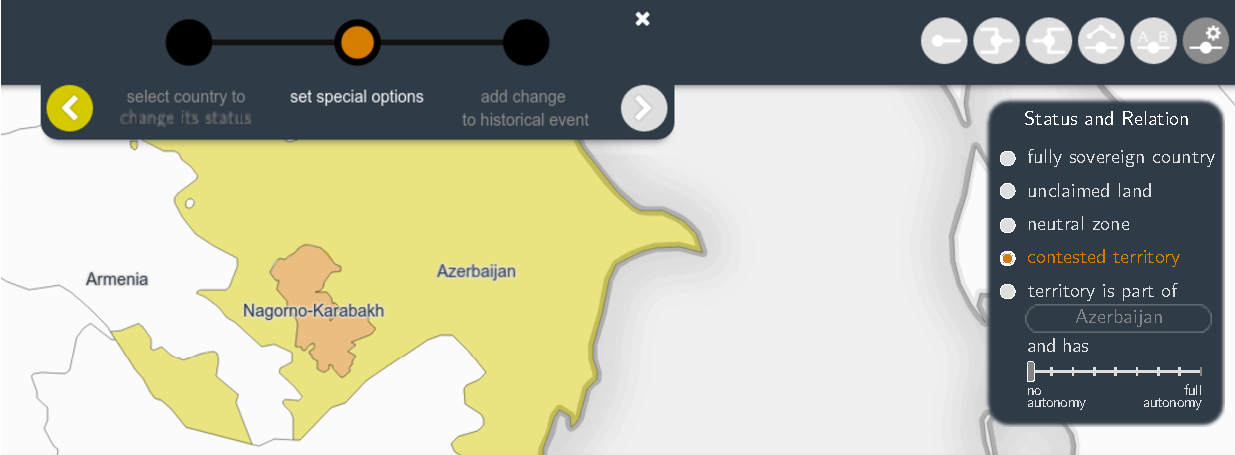
\includegraphics[width = 0.8\textwidth]{graphics/uncertainty/new_status_tool}
  \caption{Defining a special status or relationship to a territory.}
  \label{fig:uncertainty_new_status_tool}
\end{figure}

% paragraph set_new_status (end)


\paragraph{Add Historical Change} % (fold)
\label{par:add_historical_change}

The visualization of an Hivent gets split up into three parts:

\begin{enumerate}
  \item An information section storing important meta data of the event location, the dates (timespan in which the event happened), a description and the lin kto the wikipedia article (if given).
  \item A section storing all historical changes associated with that historical event. Each historical change is visualized and is assigned a date at which this event came into effect.
  \item A multimedia section stores images, videos, audio files and documents and their sources associated to the historical event.
\end{enumerate}

Similar to the extension of the area name step, also Hivent names can be chosen among a collection of Wikipedia articles describing historical events. Selecting a name from a wikipedia article automatically fills the information section and adds multimedia files from the wikipedia article. The historical change will automatically be entered in the section (see figure \ref{fig:uncertainty_new_hivent_box}). With this separation, different historical changes at different dates can be associated with one historical events, largely increasing the \texttt{Hivent} data model.

\begin{figure}[H]
  \centering
  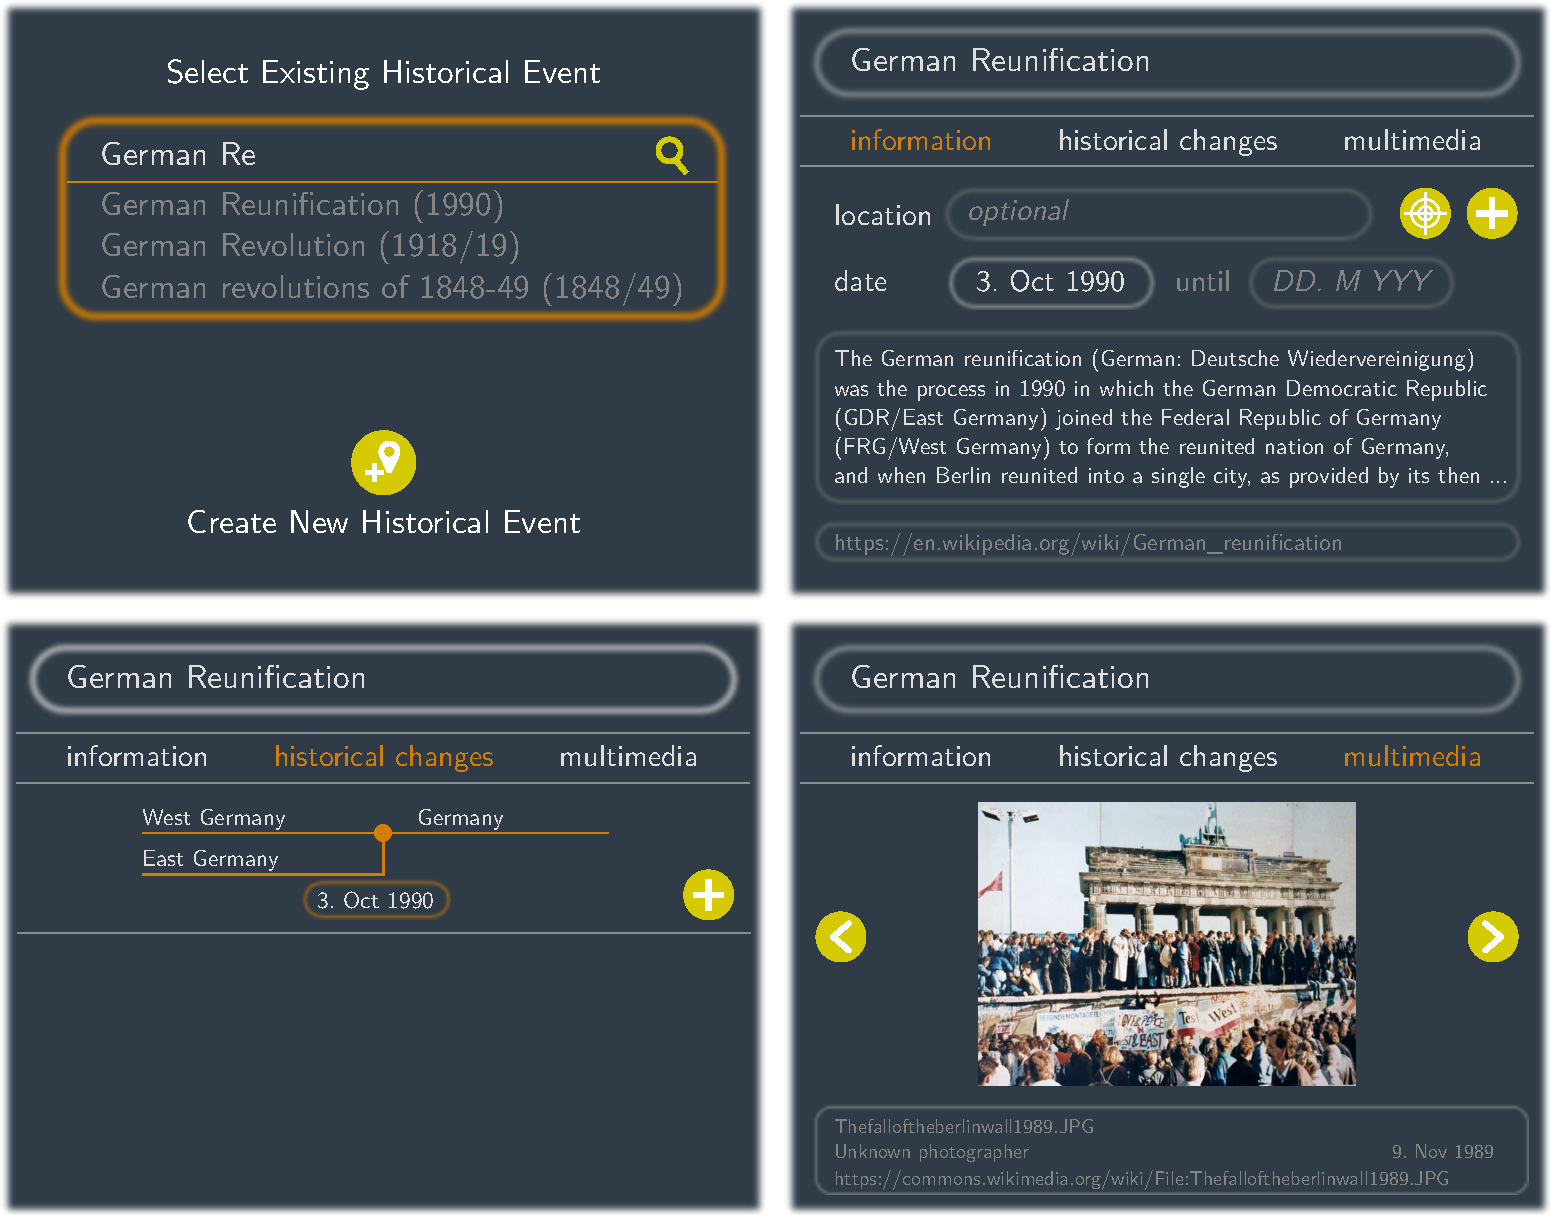
\includegraphics[width = 0.8\textwidth]{graphics/uncertainty/new_hivent_box}
  \caption{Creating a new Hivent and adding the newly created historical change.}
  \label{fig:uncertainty_new_hivent_box}
\end{figure}

% paragraph add_historical_change (end)



\paragraph{New Area Recognition} % (fold)
\label{par:new_area_recognition}

One new operation is to add the recognition of one country by another country. That is simply performed by selecting two areas on the map, whereas the first area recognized the second area. This is an historical change that can afterwards be attached to an Hivent.

\begin{figure}[H]
  \centering
  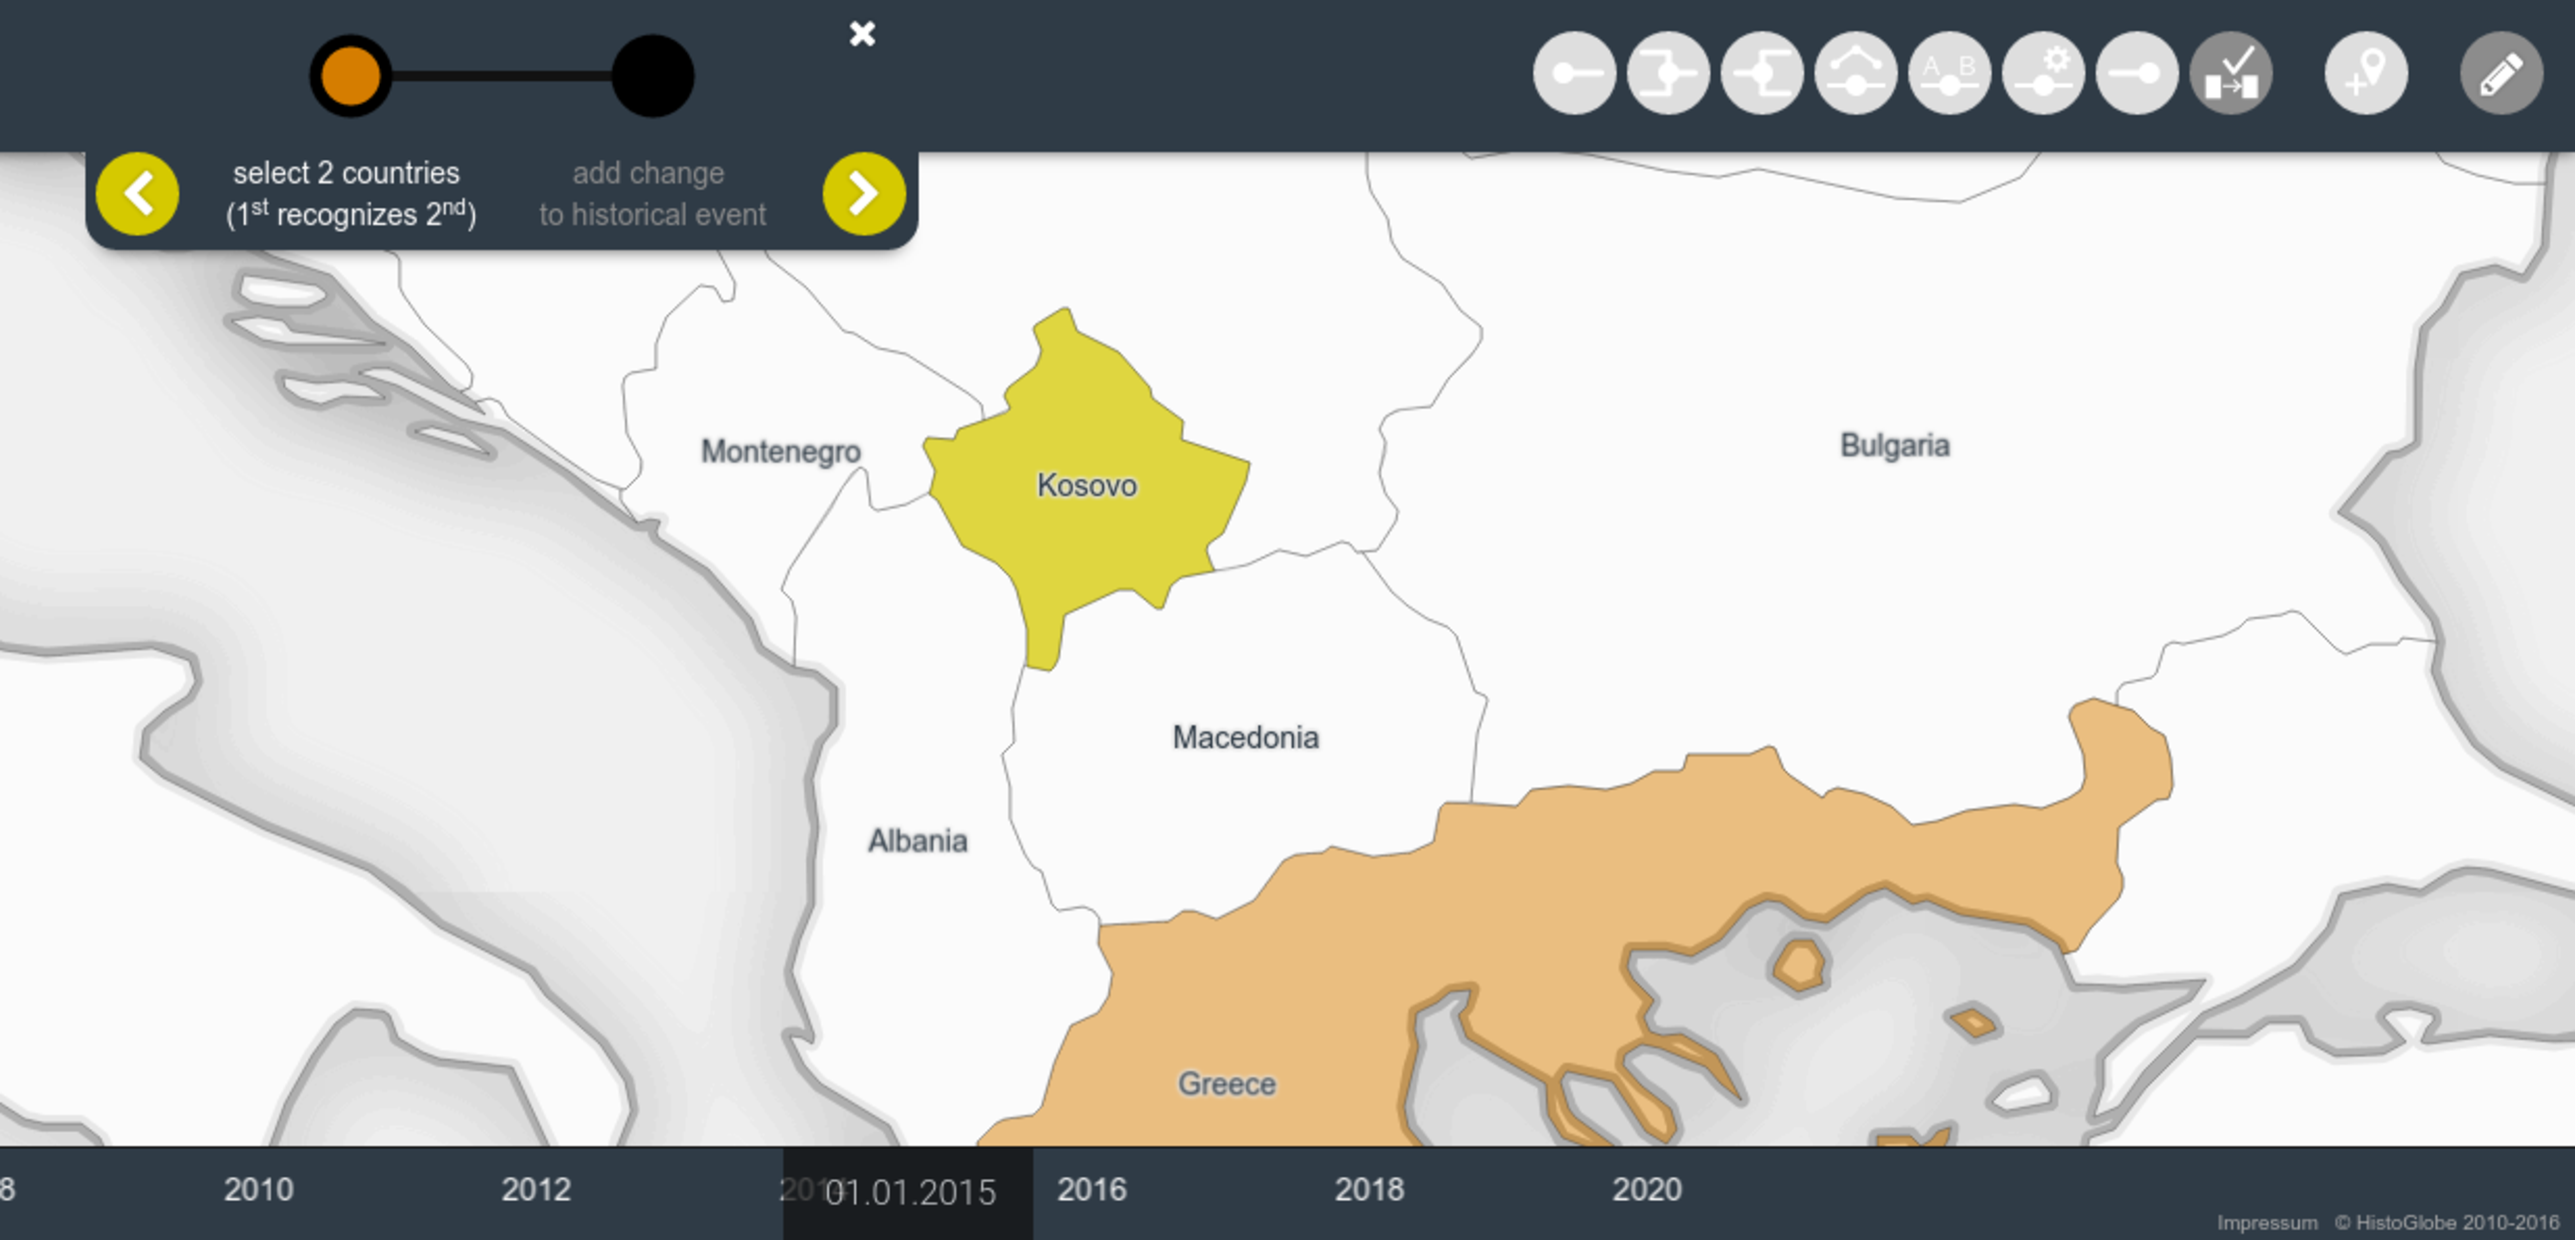
\includegraphics[width = 0.8\textwidth]{graphics/uncertainty/operation_REC}
  \caption{New edit operation: Recognition -- sets up the recognition of one area to another.}
  \label{fig:uncertainty_operation_REC}
\end{figure}


% paragraph new_area_recognition (end)

\paragraph{Multi-language support} % (fold)
\label{par:multi_language_support}

In order to support different languages, a language selection is placed on the bottom right corner of the interface, on the timeline (see figure \ref{fig:multi_language}). This changes the language of the whole interface and loads the translations of the area names and the Hivent names, locations and descriptions in the newly created language. If a term is not defined in the language, the fallback language (English) is used instead.

\begin{figure}[H]
  \centering
  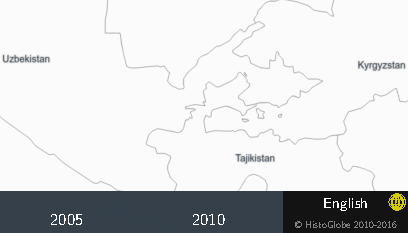
\includegraphics[width = 0.45\textwidth]{graphics/uncertainty/multi_language}
  \caption{Changing the language in the user interface.}
  \label{fig:multi_language}
\end{figure}


% paragraph multi_language_support (end)


% subsection extension_of_the_edit_mode (end)

% ------------------------------------------------------------------------------
\subsection{Extension of the Data Model} % (fold)
\label{sub:extension_of_the_data_model}

To account for the changes in the interface, also the data model has to be adapted. The main changes to the original data model developed in section \ref{cha:development} are:
% TODO: real section of original data model

\begin{enumerate}
  \item Creation of a \texttt{Multilang} entity to store a name of an Hivent, its location or an Area name in different languages.
  \item Outsourcing of the \texttt{HiventLocation} into an own entity to identify a location with a name and a geospatial reference.
  \item Creation of a \texttt{Multimedia} entity to manage multimedia files associated to an Hivent.
  \item Attachment of a date to an \texttt{HistoricalChange}.
  \item Inclusion of the \texttt{formal\_name} into the \texttt{Area} model to emphasize it as the identifier of an area.
  \item Creation of an \texttt{AreaBorder} with a \texttt{borderline}. A set of \texttt{AreaBorders} create one \texttt{AreaTerritory} which is associated to the Area. Each change of an \texttt{AreaBorder} creates one or two new \texttt{AreaTerritory}/ies.
  \item Creation of an \texttt{AreaStatus} an an \texttt{AreaRelation} to account for special status of an area alone or in relation to another area with a certain level of autonomy.
  \item Creation of an \texttt{AreaRecognition} to account for international recognition of one area to another one.
  \item Adaption of the \texttt{AreaChange} entity to model a change of each possible property of an area.
\end{enumerate}


\begin{figure}[ht]
  \centering
  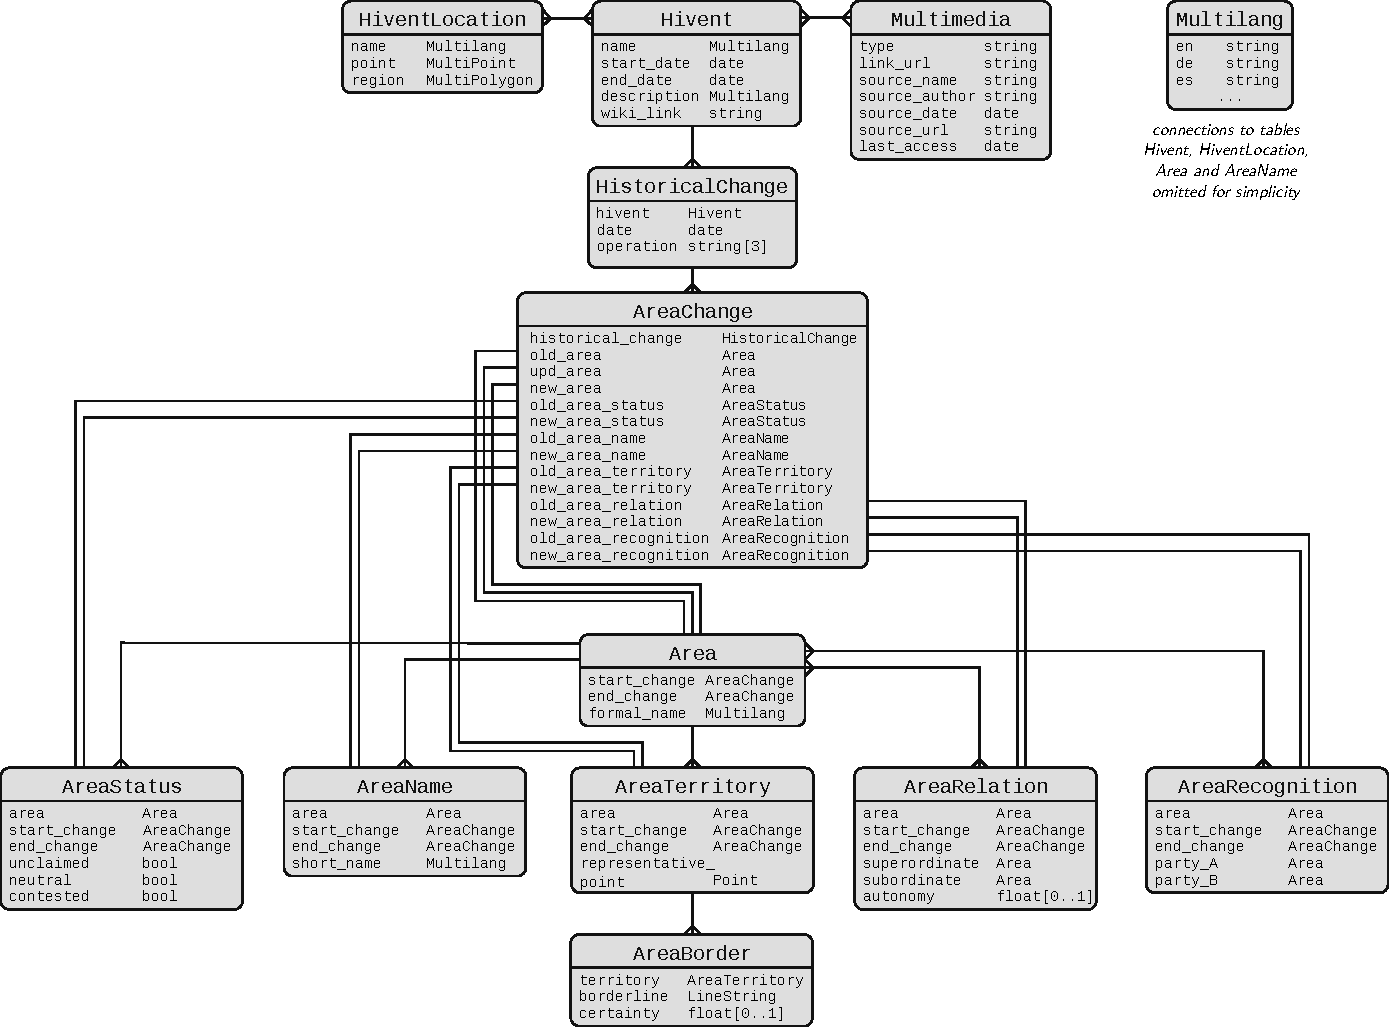
\includegraphics[width = 0.8\textwidth]{graphics/uncertainty/new_data_model}
  \caption{The new data model to support the developed approaches regarding uncertainty}
  \label{fig:new_data_model}
\end{figure}

% subsection extension_of_the_data_model (end)

% section solution_approaches (end)


% ==============================================================================

% chapter uncertainty (end)
%!TEX root = ../masters_thesis.tex

\chapter{Summary} % (fold)
\label{cha:summary}


This Master's thesis started with the motivation to lay the foundation for a Historical Geographic Information System that shows the history of countries on Earth. While there are many interesting visualizations about historical topics, wars or events, there is no such thing as an interactive historical world atlas. This may be due to the fact that there is no comprehensive collection of historical data and that the whole nature of history is that everything we know is potentially uncertain. Even the commonly accepted concept of a ``country" is impossible to define without running into conflicts. To create an information system in such a complex domain is very challenging.


% ==============================================================================
\section{Results} % (fold)
\label{sec:results}

To summarize the most important results and contributions of this Master's thesis, the four research questions are finally answered.

\begin{description}[labelindent=0.55em]
  \item[\textbf{1)}]
  \textbf{
    What type of historical changes can happen in the development of countries in time and space?
  }
\end{description}

The history of countries is very complex. The problem space of this work was limited to the territory and name of a country. Except for the coastlines, the more interesting interior borders have always changed due to sudden events. The same is true for the name of countries. If a universe $\Omega$ is defined as an ever-existing territory that initially covered the whole surface of the Earth, then this thesis has shown an interesting result: With the exception of the rare case of reincarnation, everything that has ever happened to names and territories of countries can be expressed by five basic historical changes: Unification, separation, incorporation, secession and name change.

\begin{description}[labelindent=0.1em]
  \item[\textbf{2a)}]
  \textbf{
    How can these changes be modeled in an information system?
  }
\end{description}

These five changes are modeled in the \emph{Hivent model}, an event-based spatio-temporal data model for vector data, organized by a four-domain model and visualized in a graph.
\emph{Hivents} -- \emph{\textbf{Hi}storical e\texttt{vents}} - are historically significant happenings in time.
Countries are represented by abstract \emph{Areas} with a formal name, a short name and a territory. They can change due a combination of five \emph{Hivent operations} representing exactly the five historical changes. Each operation ceases or creates a set of Areas or updates the properties of an Area.
The history of Areas can be visualized spatially on a map and non-spatially on the \emph{HistoGraph}

\begin{description}[labelindent=0.1em]
  \item[\textbf{2b)}]
  \textbf{
    How can these changes be edited by humans in a user interface?
  }
\end{description}

While the Hivent operations are very well understood by a machine, they are not suitable to be used by humans to manually edit the course of history. For that matter, six \emph{edit operations} are developed: Create, merge, split, change border, rename and cease. An edit operation can be directly performed on the map using a workflow of four steps:

\begin{compactenum}
  \item Select the Areas that will be changed in the operation.
  \item Create a territory for each new Area resulting from the operation.
  \item Create a name for each new Area.
  \item Add the edit operation to a Hivent to inherit the time stamp.
\end{compactenum}

Internally, the edit operations are expressed by a combination of the five Hivent operations and visualized on the HistoGraph. The Hivent model including the Hivent operations and the edit operations are the main contributions of this Master's thesis to the research field of spatio-temporal data models.

The model and the operations were implemented in HistoGlobe, a web-based Historical Geographic Information System that aims to visualize the history of the world on a map and a timeline. The user interface was extended by the edit mode to edit the historical data about Areas and Hivents in the system. In several user studies of the human-centered design process in this work the interface proved to be understandable and usable.

\begin{description}[labelindent=0.55em]
  \item[\textbf{3)}]
  \textbf{
    How can the model handle uncertainty and disagreement in history?
  }
\end{description}

While the initially developed Hivent model works very well given the absolute certainty about the data in the system, it has no support for any kind of imperfection, known lack of accuracy and precision or disagreement. Therefore, extensions to the original Hivent model were developed.

Areas can be assigned a special status, e.g. being a contested territory, an autonomous country within a sovereign country or a neutral zone. This will visualize the Areas differently and serve as a visual clue to signal disagreement or uncertainty. The concept of international recognition is introduced to solve the problem how to deal with questionable ``maybe'' countries: If a country has no or limited recognition by other countries, it will not be visualized the same way. The borders of Areas get an additional property that signifies the \emph{certainty} about their course. The lower the certainty, the blurrier or wider the border will appear on the map to signify limited expected accuracy.

These approaches reveal the actual problem of information systems dealing with imperfection: The user who is uncertain about the property of an object, needs to tell the information system \emph{exactly how uncertain} he or she is. That is ironically difficult.

% section results (end)

% ==============================================================================
\section{Problems and Improvements} % (fold)
\label{sec:problems}

As it has already been examined in the evaluation in section \ref{sec:evaluation}, there are several problems with the Hivent model. It has currently no support for actors -- to answer the question ``who?'' -- and for actual locations -- to say ``where?''. Both can easily be integrated and would allow new perspectives on historical events. HistoGlobe is currently only available in English. Internationalization is desired, but problematic, because in different cultures there are not just syntactically different translations, but semantically different concepts of the same historical event. This issue comes along with the desired support for different perspectives, based on different historical evidence. There is a lot of interdisciplinary research to be done in digital humanities how to support multiple perspectives on data.

The two basic assumptions about the territory of a country -- constant coastlines and a lack of sea territory -- are wrong. The Hivent model supports only sudden spatio-temporal changes due to events, but not due to gradual processes. The data model for HistoGlobe would need to be extended with a concept of \emph{Geoprocesses} that model the long-term geographical processes that lead to changing coastlines. This is an entirely different research field that would need to be entered.

Given the current status of the implementation, there is plenty of room for improvement. First of all, the design approaches developed in the previous section have to be further developed and implemented into the final system to support various degrees of uncertainty. Additionally, the information visualization problems regarding the HistoGraph have to be solved to support it in the browsing and the edit mode of HistoGlobe. The tool for semi-automatic extraction of historical maps needs to be integrated into the New Name Tool to simplify the process of creating the territory of a historical country. It also needs to support importing existing geodata in various formats. To cope with potentially more data in the database, a more sophisticated client-server interaction for initializing the state of the system needs to be developed.

However, the most crucial part is the implementation of the complicated concepts of retrospective updates and backward changes. Without them, HistoGlobe is still useless for editing the historical developments of countries in time and space. For that matter, the problem of retrospective updates needs to be further analyzed to identify possibilities for simplification. If the insertion of an update leads to more than 10 recursive updates that the user has to perform, this might be very frustrating. One idea would be to always give priority to the latest correction in case of a conflict that can be solved in two ways.

New visualization techniques can also be introduced. Animated transitions between two states of an Area would significantly increase the usability of the browsing mode. The attention of the user would be drawn to the territories that currently change. To properly account for the name of the software, a three-dimensional globe can be implemented to replace the map. This requires the use of the graphics card via \emph{WebGL}, because rendering of and interaction with a globe is much more computationally intensive than with a map. A logarithmic version of the timeline would also be interesting. A user study could analyze whether it really suits the logarithmic nature of human perception better than a normal linear timeline.

Finally, to tackle a problem of digital humanities: The current model allows to trace \emph{changes over time} and provide \emph{context}, two of the foundations of history introduced in section \ref{par:history}. However, historians do not necessarily need a tool to better visualize existing knowledge, because digital historical maps, audio or video sources are sometimes sufficient to show their results. For their research purpose it is crucial to generate new knowledge to establish \emph{causality}, another foundation for history. Therefor historians need to analyze spatio-temporal coherences or distributions in historical data by sorting, selecting or classifying the data in the system and running spatio-temporal queries. Spatio-temporal reasoning is still not easily possible with existing HGIS and yields many interesting research questions to be solved.

% section problems (end)

% ==============================================================================
\newpage
\section{Prospect} % (fold)
\label{sec:prospect}

Imagine the problems that were mentioned are solved and the room for improvement is filled with nicely designed user interface elements, then HistoGlobe would have the potential to be a well usable Historical Geographic Information System for the history of countries in time and space.

Imagine scholars in humanities use the edit mode of HistoGlobe to continuously improve the historical data in the system, animate historical countries and discuss historical events. Imagine HistoGlobe could be used not just to answer \emph{what} has happened, \emph{where} and \emph{when} did it happen and \emph{who} participated -- but to answer ultimate question \emph{why} something is the way it is?
What are the real causes for the current Syrian civil war?
Despite the conflicts in the Middle East, do we live in a peaceful time?
Why did the Roman Empire collapse?

It would help teachers to explain history to their students and learners to finally understand the seemingly complex course of history. If that would work, HistoGlobe would be a comprehensive historical world atlas with a great potential to teach, learn and understand processes in the past. We could learn from our mistakes we have done in the past and reason about the things that actually matter: To provide a world without the need for greed and hunger, for brotherhood of men. If John Lennon is right, then this information system would at some point come to its ultimate end: all countries unify to one world the common universe -- without borders. All the people living life in peace.

\vspace{2em}
\begin{large}
\begin{quoteright}
  You may say I am dreamer, \\
  but I am not the only. \\
  I hope someday you'll join us. \\
  And the world will be as one.
\end{quoteright}
\end{large}


% section prospect (end)

% ==============================================================================

% chapter summary (end)


%\* BIBLIOGRAPHY*\

% reduce font size of bibliography
{\footnotesize{
  \bibliography{chapter/sources}{}
}}
\bibliographystyle{chapter/alphaurl}


%\* APPENDIX *\

%!TEX root = ../thesis.tex

\section*{Stuff} % (fold)
\label{sec:stuff}

% section stuff (end)



\end{document}
